\documentclass[11pt,letterpaper]{report}
\usepackage[margin=1in]{geometry}
\usepackage[utf8]{inputenc}
\usepackage[T1]{fontenc}
\usepackage{helvet}
\renewcommand{\familydefault}{\sfdefault}
\linespread{1.5}
\usepackage[spanish,es-nodecimaldot]{babel}
\usepackage{titlesec}
\usepackage[hidelinks]{hyperref}
\usepackage[skip=0pt plus8pt, indent=1.25cm]{parskip}

% Formato de tabla y de título de tabla
\usepackage{graphicx}
\usepackage{caption}
\captionsetup[table]{skip=0pt,singlelinecheck=off}

\usepackage{pdfpages}
% Formatos de títulos
\titleformat{\chapter}[block]{\normalfont\fontsize{12pt}{12pt}\bfseries}{SECCIÓN \ \thechapter.}{0.6em}{\centering\MakeUppercase}
\titlespacing*{\chapter}{0em}{*3}{*2}
\titleformat{\section}[block]{\normalfont\fontsize{12pt}{12pt}\bfseries}{\thesection}{0.6em}{}
\titlespacing*{\section}{0em}{*2}{*1.2}
\titleformat{\subsection}[block]{\normalfont\bfseries\itshape}{\thesubsection}{0.6em}{}
\titlespacing*{\subsection}{4em}{*1}{*0.6}

% Formato de citación
\usepackage{csquotes}
\usepackage[backend=biber, style=vancouver]{biblatex}
\DeclareFieldFormat*{url}{\bibstring{urlfrom}: \url{#1}}
\DeclareFieldFormat{urldate}{[\bibstring{urlseen}: \space#1]}
\addbibresource{mydocument.bib}

\DefineBibliographyStrings{spanish}{
	urlfrom = {Disponible en},
	urlseen = {Accedido},
}

% Formato de numeración
\renewcommand*{\theenumi}{\thesection.\arabic{enumi}}
\renewcommand*{\theenumii}{\theenumi.\arabic{enumii}}

% Cosas generales
\title{Factores de riesgo en el neurodesarrollo infantil}
\author{Soto Consuegra, Josué Daniel \and López Castillo, Sarah Ivón \and
Ixquiac Vásquez, Etelvina Del Rosario \and Guzmán Pérez, Mariana Del Rosario
\and Mazariegos Manrique, Sonia María}
\newcommand{\tiempito}{durante mayo de 2025}
\newcommand{\muestradeseada}{1,701}
\newcommand{\asq}{“Cuestionario Edades y Etapas 3”}

\begin{document}
%	\chapter*{Dedicatoria}
%	\chapter*{Agradecimiento}
%	\chapter*{Resumen}
	\tableofcontents
%	\chapter{Introducción}
	\chapter{Planteamiento del problema}
\section{Descripción del problema}
Los trastornos del neurodesarrollo infantil representan un desafío
significativo para la salud pública en Guatemala, particularmente en regiones
como Quetzaltenango donde convergen múltiples factores de riesgo
socioeconómicos y ambientales. Según el informe de la línea de base de la Gran
Cruzada Nacional por la Nutrición 2021/2022, apenas el 49.8\% de los niños
guatemaltecos entre 24 y 59 meses se encuentran en el camino adecuado de
desarrollo, salud, aprendizaje y bienestar psicosocial. Esta situación se
agrava por el limitado acceso a programas de primera infancia, evidenciado por
el hecho de que solo el 1.9\% de las madres de niños entre 2 y 5 años
reportaron que sus hijos habían asistido alguna vez a estos programas.
\cite{SESAN2022}

En el contexto global, UNICEF reporta que aproximadamente 250 millones de niños
menores de 5 años están en riesgo de no alcanzar su potencial de desarrollo, y
cerca de 200 millones presentan retrasos en su desarrollo global debido a la
desnutrición en la primera infancia. \cite{UNICEF2023} Esta problemática se
refleja en Guatemala, donde la convergencia de factores como la pobreza, el
acceso limitado a servicios de salud y la desnutrición crónica crean
condiciones que pueden afectar negativamente el neurodesarrollo infantil.

Los estudios previos realizados en contextos similares han demostrado
asociaciones significativas entre diversos factores de riesgo y el retraso en
el desarrollo infantil. Por ejemplo, investigaciones realizadas en Etiopía han
encontrado que el retraso en el crecimiento y el bajo peso, están fuertemente
asociados con retrasos en el desarrollo. Sin embargo, existe una brecha
significativa en la investigación sobre estos factores en el contexto
específico de Quetzaltenango.

\section{Delimitación del problema}
\begin{enumerate}
	\item Ámbito geográfico: El estudio se realizará en el distrito de
		Quetzaltenango, específicamente en tres servicios de salud: el Centro
		de Salud de Quetzaltenango, el Puesto de Salud de Pacajá y el Puesto de
		Salud de San José Chiquilajá.
	\item Ámbito institucional: La investigación se desarrollará en los
		servicios de atención primaria del Ministerio de Salud Pública y
		Asistencia Social ubicados en el distrito de Quetzaltenango.
	\item Ámbito poblacional: La población de estudio comprenderá niños de 0 a
		59 meses que acuden a los servicios de atención primaria mencionados
		para controles de crecimiento y desarrollo, vacunación o consulta
		médica, excluyendo aquellos con diagnóstico previo de trastornos del
		neurodesarrollo o discapacidad intelectual.
	\item Ámbito temporal: El estudio se realizará durante el período de marzo
		a junio de 2025, tiempo durante el cual se evaluarán 1,697 niños que
		cumplan con los criterios de inclusión.
	\item Ámbito temático: La investigación se centrará en la identificación y
		análisis de los factores de riesgo asociados al neurodesarrollo
		infantil, evaluando específicamente cinco dominios mediante el
		Cuestionario Edades y Etapas 3:
		\begin{itemize}
			\item Desarrollo de la comunicación
			\item Desarrollo motor grueso
			\item Desarrollo motor fino
			\item Habilidades de resolución de problemas
			\item Desarrollo socio-individual
		\end{itemize}
\end{enumerate}

\section{Preguntas de investigación}
	\begin{enumerate}
		\item ¿Qué patrones específicos de riesgo en los dominios del
			neurodesarrollo pueden identificarse mediante el Cuestionario
			Edades y Etapas 3 en niños menores de 5 años que asisten a
			servicios de atención primaria en Quetzaltenango?
		\item ¿Cuál es la asociación entre factores socioeconómicos,
			demográficos, familiares y antecedentes perinatales con el riesgo
			de retraso en cada uno de los cinco dominios del neurodesarrollo
			evaluados mediante el ASQ-3 en niños menores de 5 años en
			Quetzaltenango?
		\item ¿En qué medida el acceso a servicios de atención primaria durante
			los períodos prenatal y postnatal modifica la asociación entre
			factores de riesgo socioeconómicos y el desarrollo infantil
			temprano en los distintos dominios evaluados por el Cuestionario
			Edades y Etapas 3?
	\end{enumerate}

	\chapter{Objetivos}
\section{Objetivo general}
	\begin{enumerate}
		\item Establecer la asociación entre factores sociodemográficos,
		económicos, familiares y médicos con el riesgo en el neurodesarrollo en
		niños menores de 5 años que asisten a servicios de atención primaria en
		el distrito de Quetzaltenango, mediante evaluaciones con el \asq\
		durante 2025.
	\end{enumerate}
\section{Objetivos específicos}
	\begin{enumerate}
		\item Clasificar los resultados del \asq\ según grupos de edad para
		detectar patrones específicos de riesgo en los dominios del
		neurodesarrollo.
		
		\item Evaluar la asociación entre factores socioeconómicos,
		demográficos, ambientales y antecedentes perinatales y el riesgo de
		retraso en el neurodesarrollo utilizando el \asq.
		
		\item Analizar la relación entre acceso a servicios de atención
		primaria durante el periodo prenatal y postnatal con la presencia de
		riesgo de retraso en el neurodesarrollo.
	\end{enumerate}

	\chapter{Justificación}
Los trastornos del desarrollo, también conocidos como retrasos del desarrollo,
constituyen un grupo heterogéneo de condiciones que afectan el aprendizaje, el
lenguaje, el comportamiento o las habilidades motoras.
\cite{cdcDevelopmentalDisability} Estos retrasos se identifican cuando un niño
no alcanza los hitos de desarrollo esperados en comparación con sus pares de la
misma población \cite{DevelopmentalSurveillance}. Por ello es importante
destacar que el retraso en el desarrollo no es un diagnóstico en sí mismo, sino
un término descriptivo utilizado en la práctica clínica para indicar un
fenotipo amplio que requiere una evaluación más detallada para determinar las
áreas específicas de desarrollo afectadas. Hay tres tipos de retraso en el
desarrollo basado en el número de dominios involucrados: 1) Retraso aislado en
el desarrollo: involucra un solo dominio; 2) Múltiples retrasos en el
desarrollo: 2 o más dominios o líneas de desarrollo afectados; y, 3) Retraso
global en el desarrollo: retraso significativo en la mayoría de los dominios de
desarrollo. \cite{Bellman2013} Aunque la etiología de la mayoría de los
retrasos en el desarrollo es idiopática, cuando se identifica, puede incluir
factores genéticos, ambientales y/o psicosociales. \cite{DevelopmentalDelay}

En Guatemala, según el informe de la línea de base de la Gran Cruzada Nacional
por la Nutrición 2021/2022 de la Secretaría de Seguridad Alimentaria y
Nutricional, solo el 1.9\% de las madres de niños entre 2 y 5 años reportaron
que sus hijos habían asistido alguna vez a un programa de primera infancia, y
apenas el 0.6\% asiste actualmente a un Centro Comunitario de Desarrollo
Infantil Temprano. Más preocupante aún, solo el 49.8\% de los niños de 24 a 59
meses se encuentran en el camino adecuado de desarrollo, salud, aprendizaje y
bienestar psicosocial. \cite{SESAN2022}

A nivel global, según un reporte de UNICEF en 2023, se estima que 250 millones
de niños menores de 5 años están en riesgo de no alcanzar su potencial de
desarrollo. Aproximadamente 200 millones de niños menores de 5 años no están
creciendo, no presentan un adecuado desarrollo global, debido a la desnutrición
en la primera infancia. Además, más de 2 de cada 5 niños entre 3 y 4 años no
reciben la estimulación temprana ni el cuidado parental adecuados. Como
resultado de estas y otras amenazas, el 29\% de los niños de 3 a 5 años no
están logrando un desarrollo apropiado. \cite{UNICEF2023}

El neurodesarrollo infantil es un proceso complejo y dinámico que sienta las
bases para el futuro cognitivo, emocional y social de los individuos. En
Quetzaltenango, Guatemala, existe una brecha significativa en la investigación
sobre los factores que influyen en el desarrollo neurológico de los niños
menores de 5 años. Esta carencia de datos locales específicos obstaculizan la
implementación de intervenciones efectivas y políticas públicas adecuadas.

Para llevar a cabo este estudio en Quetzaltenango, es necesario un equipo de 5
investigadores debido a la complejidad y el alcance de la muestra, la cual
comprende \muestradeseada\ niños. La distribución del trabajo se detalla a
continuación:

	\begin{itemize}
		\item Carga de trabajo y distribución: Cada investigador estará a cargo
		de evaluar aproximadamente 340 niños, lo cual permite una división
		equitativa para asegurar una atención detallada en cada caso. Esto es
		crucial para mantener la calidad de los datos y la consistencia en la
		recolección de información, aspecto necesario para la validez del
		estudio.
		\item Tiempo estimado de evaluación: Cada evaluación individual tomará
		alrededor de 30 a 50 minutos. Esto representa aproximadamente 1,417
		horas en total o 283 horas por investigador. La presencia de 5
		investigadores optimiza el proceso y asegura que las evaluaciones se
		realicen en el tiempo programado.
		\item Cobertura de múltiples puntos de atención: La investigación se
		llevará a cabo en tres servicios de atención primaria de
		Quetzaltenango: el Centro de Salud de Quetzaltenango, el Puesto de
		Salud de Pacajá y el Puesto de Salud de San José Chiquilajá.
		\item Atención a casos en riesgo: Los niños identificados con riesgo en
		el neurodesarrollo y sus padres o tutores recibirán plan educacional y
		material de apoyo para promover actividades de estimulación temprana en
		casa. El mismo lo llevará a cabo el investigador utilizando
		herramientas recomendadas por UNICEF.
	\end{itemize}

En conclusión, la integración de un equipo de 5 investigadores permite abordar
de manera exhaustiva y precisa los desafíos de la evaluación de neurodesarrollo
en niños menores de 5 años en Quetzaltenango. Los resultados esperados no solo
aportarán evidencia científica local, sino que también promoverán
intervenciones que puedan mejorar el desarrollo integral de los niños,
sensibilizando a las autoridades y profesionales de la salud sobre la
importancia de intervenciones tempranas y costo efectivas en el desarrollo de
la primera infancia.

	\chapter{Marco teórico}
\section{Antecedentes y contextualización del neurodesarrollo infantil}
\subsection{Panorama global del desarrollo infantil}
A nivel global,  los desafíos asociados con el desarrollo infantil son amplios
y están influenciados por factores socioeconómicos, culturales y ambientales.
Según UNICEF, aproximadamente 250 millones de niños menores de 5 años están en 
riesgo de no alcanzar su potencial de desarrollo debido a factores como la 
desnutrición, la falta de estimulación temprana y el acceso limitado a 
servicios de salud y educación \cite{UNICEF2023}. Estas condiciones adversas 
son particularmente prevalentes en países de ingresos bajos y medios, donde se 
observan altas tasas de desnutrición crónica y pobreza.

La neurociencia del desarrollo ha demostrado que los primeros años de vida, 
especialmente los primeros 1000 días, son críticos para el desarrollo cerebral. 
Durante este período, las experiencias ambientales y las interacciones con los 
cuidadores moldean la arquitectura del cerebro, impactando habilidades como el 
lenguaje, la memoria y el control emocional \cite{Stiles2010}. Las adversidades 
tempranas, como la pobreza y la desnutrición, pueden tener efectos negativos 
duraderos en la plasticidad cerebral, lo que subraya la importancia de 
intervenciones tempranas y programas de estimulación.

Desde una perspectiva ecológica, el desarrollo infantil está influenciado por 
múltiples sistemas que interactúan entre sí, como se describe en el modelo de 
Bronfenbrenner \cite{Bronfenbrenner2005}. Este enfoque destaca la importancia 
de los entornos inmediatos, como la familia y la comunidad, así como de 
factores más amplios, como las políticas públicas y las normas culturales. Por 
ejemplo, en Guatemala, el acceso limitado a programas de primera infancia y los 
altos índices de desnutrición crónica limitan significativamente las 
oportunidades de desarrollo infantil, especialmente en comunidades rurales 
\cite{SESAN2022}.

\subsection{Contexto guatemalteco del neurodesarrollo infantil}
Guatemala se caracteriza por ser un país con una rica diversidad cultural,
conformado por diferentes grupos étnicos: Maya, Garífuna, Xinka y Mestizo. 
Aunque la mayoría de la población guatemalteca (54\%) reside en zonas urbanas,
es importante señalar que la población indígena habita predominantemente en
áreas rurales (57\%). \cite{PoliticaInfanciaGuate}

El panorama demográfico de Guatemala presenta importantes desafíos para la
primera infancia. Según datos del censo poblacional de 2018, en el país habitan
aproximadamente 2,3 millones de niñas y niños menores de 6 años, de los cuales
cerca de un millón viven en condiciones de pobreza y 800 mil en situación de
extrema pobreza. \cite{INE} Los departamentos con mayor proporción de población
infantil temprana son Totonicapán (41.7\%), Huehuetenango (41.4\%) y El Quiché
(41.1\%). \cite{UNICEFAtlas} Adicionalmente, el 3.8\% de la población infantil
y adolescente entre 4 y 17 años presenta algún tipo de dificultad visual,
auditiva, física, de concentración, autocuidado o comunicación. \cite{INE}

Si bien Guatemala constituye la economía más grande de América Central en
términos de población (aproximadamente 17.6 millones de habitantes en 2023) y
actividad económica (con un PIB de 104.4 mil millones de dólares
estadounidenses en 2023), este crecimiento económico no se ha traducido en una
reducción significativa de la pobreza. Para 2023, se estimaba que el 55\% de la
población vivía en condiciones de pobreza, mientras que la economía informal
representaba el 49\% del PIB, con un 71.1\% de la población empleada trabajando
en el sector informal. \cite{WorldBankGuate} Es importante destacar que la
pobreza y las experiencias adversas durante la infancia tienen efectos
fisiológicos y epigenéticos a largo plazo en el desarrollo cerebral y la
cognición. \cite{Luby_2015} \cite{Noble_2015}

La situación del desarrollo infantil en Guatemala es preocupante. De acuerdo
con los datos de 2021-2022, Guatemala ha obtenido un 50\% en el Índice de
Desarrollo Infantil Temprano, lo que significa que apenas la mitad de los niños
entre 24 y 59 meses presenta un desarrollo adecuado en salud, aprendizaje y
bienestar psicosocial. Existen disparidades significativas entre diferentes
grupos poblacionales: mientras que el 57.9\% de los niños no indígenas muestra
un desarrollo adecuado, solo el 45\% de los niños indígenas alcanza este nivel.
\cite{SESAN2022} Las diferencias se acentúan aún más cuando se analiza el
índice en función de la riqueza del hogar, observándose una brecha de 23 puntos
porcentuales entre los hogares con mayor y menor riqueza. \cite{UNICEFGuate}

El limitado acceso a oportunidades educativas constituye otro desafío
fundamental. En 2020, la tasa neta de cobertura en el nivel inicial fue de
apenas el 1.1\% a nivel nacional. En ese mismo año, se registraron 597,195
niñas y niños inscritos en educación preprimaria, con una cobertura nacional
del 60.8\%, representando el 13.8\% del total de estudiantes inscritos en
los distintos niveles educativos. \cite{PoliticaInfanciaGuate} Para niños
menores de 4 años, la cobertura educativa es particularmente baja, mientras que
para niños entre 4 y 6 años alcanza el 64.4\%. \cite{MineducEstadistica}

La situación educativa de la niñez con discapacidad representa un desafío
particular para el país. Según la ENDIS 2016, el 76\% de las niñas y niños
entre 5 y 18 años con algún tipo de discapacidad asiste a la escuela,
observándose una marcada diferencia entre el área urbana (90\%) y el área rural
(61\%). Los niños con limitaciones significativas en el funcionamiento físico o
cognitivo tienen menor probabilidad de ser inscritos en establecimientos
educativos. \cite{PoliticaInfanciaGuate}

Al analizar la relación entre desarrollo infantil temprano y estado
nutricional, los resultados son consistentes con estudios previos que
demuestran que los niños con desnutrición crónica tienden a presentar un menor
desarrollo. En la encuesta de línea base de la Cruzada Nacional por la
Nutrición 2021/2022, esta relación se evidencia claramente: el porcentaje de
niños con desarrollo adecuado es mayor entre aquellos que no presentan
desnutrición crónica (55,6\%) en comparación con quienes padecen este tipo de
malnutrición (43,3\%). \cite{SESAN2022}

La desnutrición crónica afecta aproximadamente al 46.5\% de los niños
guatemaltecos menores de 5 años, reflejando profundas desigualdades sociales.
El porcentaje de desnutrición crónica es significativamente mayor en áreas
rurales (53\% frente a 34.6\% en zonas urbanas), en población indígena (58\%
frente a 34.2\% en población no indígena), en hogares donde las madres carecen
de escolaridad (67.0\% frente a 19.1\% en hogares donde la madre tiene
educación superior), en hogares con menor riqueza económica (65.9\% en el
quintil inferior frente a 17.4\% en el quintil superior) y cuando existe un
menor espaciamiento entre embarazos (57.0\% frente a 39.6\% con mayor
espaciamiento). \cite{EnMaternoInfantil}

Las prácticas de alimentación infantil también presentan importantes desafíos.
Solo el 63.1\% de las niñas y niños reciben lactancia materna dentro de la
primera hora de nacidos, el 53.2\% reciben lactancia materna exclusiva entre
los 0 y 6 meses de edad, y la duración promedio de la lactancia materna
exclusiva es de apenas 2.8 meses. En cuanto a la alimentación complementaria,
el 55.7\% de los niños entre 6 y 23 meses que son amamantados reciben cuatro o
más grupos de alimentos, mientras que el 71.2\% de los niños no amamantados en
este mismo rango de edad reciben una frecuencia mínima de comidas.
\cite{EnMaternoInfantil} \cite{PoliticaInfanciaGuate}

A pesar de que el vínculo entre el cuidador y el niño es fundamental para un
desarrollo infantil positivo, muchos niños guatemaltecos experimentan violencia
por parte de sus cuidadores. Un estudio realizado a finales de 2019 en 52
comunidades de los departamentos de Sololá, Alta Verapaz, Baja Verapaz,
Chimaltenango, Quetzaltenango y San Marcos reveló que 8 de cada 10 adultos
consideran que en su comunidad la forma más habitual de corregir a los hijos es
mediante castigos físicos como cincho, chicote, vara, golpes o gritos. La mitad
de los adultos piensa que la falta de este tipo de disciplina refleja una
carencia de carácter por parte de los padres. \cite{PoliticaInfanciaGuate}
\cite{UNICEFComportamientosNinez}

\subsection{Estudios previos sobre factores de riesgo en el neurodesarrollo}
En un estudio transversal realizado por Mehner et al. (2019), titulado
``La asociación de la puntuación de riesgo acumulativo con los resultados de
ASQ-3 en una región rural empobrecida de Guatemala'', se evaluó una muestra de
conveniencia de 148 madres con niños de 12 a 52 meses de edad en una zona rural
de Guatemala. El objetivo principal fue desarrollar una puntuación de riesgo
compuesta por factores fácilmente obtenibles para diseñar intervenciones e
identificar a los niños de alto riesgo que más se beneficiarían de estas. Se
utilizaron encuestas de interacción madre-hijo y \asq\ para evaluar el
desarrollo. Los resultados mostraron que el 58\% de los niños tenían
puntuaciones anormales en $\ge$1 dominio del ASQ-3, y el 35\% en $\ge$2
dominios. Se desarrollaron tres puntuaciones de riesgo: Riesgo Demográfico
Materno (DR), Interacción Madre-Hijo (MCI) y Riesgo Combinado (CR). La
probabilidad de tener $\ge$2 dominios con puntuaciones anormales aumentó
significativamente con un puntaje DR creciente (OR, 1.46 [IC 95\%, 1.15-1.86]
p<0.05) y un puntaje CR creciente (OR, 2.08 [IC 95\%, 1.41-3.07], p<0.05). Los
autores concluyeron que un índice de riesgo acumulativo combinado de factores
demográficos e interacciones madre-hijo parece ser una herramienta útil para
predecir qué niños tienen puntuaciones anormales en múltiples dominios del
desarrollo. \cite{CMehner2019}

En el contexto específico de Guatemala, un análisis del informe de la  línea de
base de la Gran Cruzada Nacional por la Nutrición 2021/2022 revela  datos
preocupantes: la cobertura de programas de primera infancia es extremadamente
limitada, con apenas un 1.9\% de niños entre 2 y 5 años que han asistido alguna
vez a estos programas. Más alarmante aún es que solo el 49.8\% de los niños
guatemaltecos entre 24 y 59 meses muestran un desarrollo adecuado  en las
dimensiones de salud, aprendizaje y bienestar psicosocial \cite{SESAN2022}.
Estos datos son consistentes con las observaciones de Mehner et al.
\cite{CMehner2019} en zonas rurales de Guatemala, donde encontraron que el 58\%
de los niños evaluados presentaban puntuaciones anormales en al menos un
dominio del ASQ-3.

En una revisión sistemática y meta-análisis realizada por Wondmagegn et al.
(2024), titulada ``Prevalencia y determinantes del retraso del desarrollo entre
los niños en países de ingresos bajos y medios: una revisión sistemática y un
metanálisis'', se analizaron 21 estudios primarios publicados entre 2010 y
2024, involucrando a un total de 54,067 niños en países de ingresos bajos y
medios. El objetivo principal fue evaluar la prevalencia combinada del retraso
del desarrollo confirmado y sus determinantes entre los niños en estos países.
Los resultados mostraron una prevalencia combinada de retraso del desarrollo
del 18.83\% (IC 95\%: 15.53-22.12\%). En el análisis de subgrupos, se observó
una alta prevalencia de retraso del desarrollo [26.69\% (IC 95\%: 15.78-37.60)]
en estudios realizados en África. Los determinantes significativos del retraso
del desarrollo fueron la educación materna [OR: 3.04; IC 95\% (2.05, 4.52)] y
el bajo peso al nacer [OR: 3.61; IC 95\% (1.72, 7.57)]. Los autores concluyeron
que la prevalencia combinada de retraso del desarrollo en países de ingresos
bajos y medios era alta en comparación con los países de altos ingresos,
especialmente en África, y que el nivel educativo materno y el peso al nacer
estaban significativamente asociados con los retrasos del desarrollo.
\cite{Wondmagegn2024}

En un estudio transversal comunitario realizado en áreas urbanas de Etiopía por
Delbiso et al. (2024), titulado ``Desarrollo de la primera infancia y estado
nutricional en la Etiopía urbana'', se evaluaron 627 pares de madres e hijos de
12-36 meses de edad entre julio y septiembre de 2022. El desarrollo infantil
temprano (DIT) se evaluó utilizando el \asq, mientras que el estado nutricional
se determinó mediante mediciones antropométricas. Los resultados mostraron que
los retrasos en los dominios del DIT eran comunes, especialmente en el dominio
motor fino (41.9\%). Más de la mitad de los niños (52.8\%) presentaban retraso
en el crecimiento. Se encontró que el retraso en el crecimiento y el bajo peso
estaban asociados con retrasos en el DIT, mientras que la desnutrición aguda no
lo estaba. Los niños con retraso en el crecimiento tenían más probabilidades de
tener peores retrasos en el DIT en los dominios motor fino (OR = 1.54; IC 95\%:
1.11-2.15), motor grueso (OR = 1.47;IC 95\%: 1.05-2.04) y resolución de
problemas (OR = 1.41; IC 95\%: 1.02-1.96) en comparación con los niños sin
retraso en el crecimiento. De manera similar, los niños con bajo peso tenían
más probabilidades de tener peores retrasos en el DIT en los dominios motor
grueso (OR = 1.91; IC 95\%: 1.20-3.04) y motor fino (OR = 1.90; IC 95\%:
1.15-3.15) en comparación con los niños de peso normal. \cite{Delbiso2024}

Domek et al. (2023) realizaron un estudio piloto para evaluar los efectos a
largo plazo de una intervención simple con títeres de dedo para promover el
desarrollo infantil temprano en el ámbito de atención primaria. La muestra
incluyó 172 niños de familias principalmente de bajos ingresos, divididos en
cohortes de intervención temprana (2 meses) y tardía (6 o 12 meses). Se utilizó
el \asq\ para evaluar el desarrollo infantil hasta los 36 meses. Los resultados
mostraron que la intervención temprana se asoció con mejores trayectorias de
desarrollo socioemocional en comparación con
la intervención tardía (diferencia en pendiente de 0.12, p=0.018). También se
observaron diferencias que se acercaron a la significancia estadística en
comunicación (p=0.056) y en la puntuación combinada no motora (p=0.052). No se
encontraron diferencias significativas en los dominios de resolución de
problemas, motricidad gruesa y fina. Los autores concluyeron que la
intervención con títeres de dedo puede proporcionar una forma simple, de bajo
costo y escalable de fomentar interacciones cuidador-infante que promuevan el
desarrollo del lenguaje y socioemocional, especialmente cuando se proporciona
en la infancia temprana. Este estudio destaca la importancia de las
intervenciones tempranas en atención primaria y su potencial impacto en el
desarrollo infantil a largo plazo. \cite{Domek2023}

En un estudio transversal, descriptivo y exploratorio realizado por Ramos y
Della Barba (2021), titulado Cuestionarios de edades y etapas de Brasil en el
seguimiento del desarrollo en la primera infancia, se analizaron 392 niños de 
5 a 50 meses de edad que asistían a 6 Centros de Educación Infantil (CEIs) en
un municipio del interior del estado de São Paulo, Brasil. El objetivo
principal fue delinear el perfil del desarrollo global de los niños utilizando 
el \asq\ edición Brasil (ASQ-BR) y verificar la aplicabilidad
de este instrumento por parte de los maestros preescolares. Los resultados
mostraron que la mayoría de los niños presentaron un desarrollo dentro de lo 
esperado, con los mejores desempeños en los dominios de Motricidad Gruesa
(79.44\%), Comunicación (72.34\%) y Resolución de Problemas (69.54\%). Sin
embargo, se observó una incidencia significativa de riesgo en los dominios
Personal-Social (22.08\%) y Motricidad Fina (19.03\%). En el análisis por sexo,
las niñas obtuvieron puntuaciones significativamente más altas que los niños en
los dominios de Motricidad Fina y Personal-Social. Los autores concluyeron que
el ASQ-BR se presenta como un instrumento potencial para el cribado del
desarrollo infantil en guarderías y preescolares, permitiendo a los
profesionales reflexionar sobre su propia práctica y atender mejor las
necesidades individuales de los niños. \cite{RAMOS2021}

Oumer et al. (2022), titulado “El retardo de crecimiento y bajo peso, pero no
la desnutrición aguda, están asociados con el retraso en el desarrollo
infantil en el suroeste de Etiopía”, se analizaron 507 pares de madres e hijos
en el Suroeste de Etiopía. El objetivo principal fue identificar la relación
entre diferentes formas de malnutrición y el retraso en el desarrollo infantil
entre niños de 12 a 59 meses de edad. Los resultados mostraron una prevalencia
de retraso en el desarrollo del 29.4\% (IC 95\%: 25.4-33.4\%). En el análisis
de subgrupos, se observaron retrasos en el desarrollo de habilidades motoras
gruesas (17.2\%), comunicación (16.8\%), resolución de problemas (13.4\%),
habilidades personales-sociales (10.8\%) y motricidad fina (10.1\%).
Los determinantes significativos del retraso en el desarrollo fueron el trabajo
materno fuera del hogar [AOR: 2.9; IC 95\% (1.8, 4.8)], el nacimiento prematuro
[AOR: 3.2; IC 95\% (1.4, 7.0)], la iniciación temprana de la alimentación
complementaria [AOR: 2.5; IC 95\% (1.37, 4.6)], el retraso en el crecimiento
[AOR: 3.0; IC 95\% (1.9, 4.7)], el bajo peso [AOR: 2.3; IC 95\% (1.1, 4.7)] y
una baja puntuación de diversidad dietética [AOR: 3.1; IC 95\% (1.3, 7.5)].
Los autores concluyeron que el retraso en el desarrollo infantil es un problema
de salud pública en la región y está fuertemente asociado con la desnutrición
crónica, el bajo peso, el consumo de una dieta poco diversificada y prácticas
subóptimas de alimentación infantil.
\cite{Oumer2022}

\subsection{Brechas en el conocimiento e importancia del estudio actual}
En el distrito de Quetzaltenango, Guatemala, la vulnerabilidad económica, el
acceso limitado a servicios de salud y los factores nutricionales representan
un riesgo significativo para el neurodesarrollo infantil. Al igual que en otros
países de ingresos bajos y medios, las condiciones adversas en esta región
pueden influir negativamente en los hitos del desarrollo infantil temprano.

Esta problemática local se enmarca en un contexto global igualmente 
preocupante. Según UNICEF\cite{UNICEF2023}, aproximadamente 250 millones de 
niños menores de 5 años a nivel mundial están en riesgo de no alcanzar su 
potencial de desarrollo, con cerca de 200 millones afectados por desnutrición 
en la primera infancia. Particularmente relevante para nuestro estudio es que 
más de 2 de cada 5 niños entre 3 y 4 años no reciben la estimulación temprana 
ni el cuidado parental adecuados, factores que Domek et al.\cite{Domek2023} 
identificaron como críticos para el desarrollo del lenguaje y socioemocional. 

La unión de los datos nacionales con los hallazgos globales subraya la 
necesidad de investigaciones específicas en contextos como Quetzaltenango, 
donde factores socioeconómicos, nutricionales y de acceso a servicios de salud 
pueden influir significativamente en los patrones de desarrollo infantil.

\section{Conceptos fundamentales del desarrollo infantil}
\subsection{Neurodesarrollo}
El neurodesarrollo es un proceso dinámico y continuo que se extiende desde 
las primeras etapas de la vida intrauterina hasta la adultez, abarcando una 
compleja interacción de factores genéticos, epigenéticos, ambientales y 
sociales. Este proceso es fundamental para el establecimiento de las bases 
cognitivas, emocionales, motoras y sociales de los individuos, las cuales 
son esenciales para su aprendizaje, adaptación y productividad a lo largo 
de la vida \cite{Stiles2010, Nelson49}.

El desarrollo cerebral está regulado por una interacción entre la expresión 
genética y las influencias ambientales. Mientras que los genes proporcionan 
el marco básico para el desarrollo de estructuras neuronales, las 
experiencias tempranas y las interacciones sociales desempeñan un papel 
crítico en la modelación de las conexiones sinápticas y en la poda neuronal. 
Como señala Stiles \cite{Stiles2010}, ``tanto la expresión genética como los
estímulos ambientales son esenciales para el desarrollo cerebral normal, y la
alteración de cualquiera de estos factores puede modificar fundamentalmente los
resultados neurales''. Estos mecanismos epigenéticos, como la metilación del
ADN, permiten que el entorno modifique la expresión genética sin alterar la
secuencia del ADN,  impactando así el desarrollo cerebral y la consolidación de
habilidades cognitivas y emocionales \cite{Roth2011, Feldman2}.

En el aspecto biológico, el neurodesarrollo durante los primeros años de vida
representa un período crítico caracterizado por un desarrollo acelerado, 
durante el cual numerosas estructuras neuronales se construyen y organizan 
siguiendo las siete fases fundamentales del desarrollo cerebral: nacimiento 
celular, migración celular, diferenciación celular, maduración celular, 
sinaptogénesis, muerte celular y poda sináptica, y mielinización.
\cite{Kolb7}

El neurodesarrollo abarca diversos dominios neurológicos fundamentales que 
evolucionan siguiendo trayectorias interconectadas: sensorial, motor grueso y
fino, lingüístico, visuo-espacial, intelectual, memoria, cognición social y
función ejecutiva. La maduración de estos dominios sigue una secuencia
relativamente predecible, aunque con  variaciones individuales significativas,
que se manifiesta a través de la  adquisición de habilidades cada vez más
complejas y refinadas. \cite{Nelson49}

\section{Procesos biológicos del desarrollo cerebral}
El cerebro humano evoluciona a partir de un grupo limitado de células
embrionarias hasta convertirse en el sistema orgánico más complejo, todo ello
durante los escasos 280 días que comprende la gestación humana. Lo que 
distingue principalmente el desarrollo fetal humano del de otras especies es 
precisamente el cerebro, con su masiva corteza prefrontal y su extraordinaria 
capacidad para investigar y reflexionar sobre su propia naturaleza y 
funcionamiento. \cite{Polin124}

Durante el neurodesarrollo, los eventos genéticos y epigenéticos se entrelazan 
siguiendo una regulación estricta, tanto temporal como espacial, transformando
un delgado disco de neuroepitelio indiferenciado en un sofisticado sistema de
múltiples capas. \cite{Polin124}

El proceso de desarrollo cerebral, genéticamente predeterminado, comprende
siete fases claramente definidas que se despliegan a lo largo de un extenso
período evolutivo. \cite{Kolb7} Mientras algunas de estas fases están
circunscritas a períodos específicos, otras mantienen su actividad durante
intervalos temporales más prolongados. Las características de estas fases se
sintetizan en el cuadro \ref{tab:fases-desarrollo-cerebral}.

\begin{table}[htbp]
\caption{Siete fases del desarrollo cerebral}
\label{tab:fases-desarrollo-cerebral}
\resizebox{\textwidth}{!}{%
\begin{tabular}{ll}
\hline
\multicolumn{1}{c}{\textbf{Fase del desarrollo}} & \multicolumn{1}{c}{\textbf{Proceso}} \\ \hline
1. Nacimiento celular & Origen de las neuronas y la glia \\
2. Migración celular & Movimiento de las células a su posición funcional \\
3. Diferenciación celular & Las células precursoras se transforman en un tipo de célula especializada \\
4. Maduración celular & Crecimiento de dendritas y axones \\
5. Sinaptogénesis & Formación de sitios de comunicación de célula a célula \\
6. Muerte celular y poda sináptica & Muerte celular programada y desmantelamiento de circuitos no usados \\
7. Mielinización & Formación de la vaina de mielina que aumenta la velocidad de neurotransmisión \\ \hline \hline
\footnotesize Modificado de: Kolb, B y Whishaw, I y Campbell T. \cite{Kolb7}
\end{tabular}%
}
\end{table}

\subsection{Desarrollo cerebral en el período embrionario}
\subsubsection{Gastrulación: establecimiento de las capas germinales primordiales}
Uno de los primeros pasos cruciales en el desarrollo cerebral ocurre durante la
tercer semana de gestación, cuando la masa celular interna bilaminar, compuesta
por el epiblasto y el hipoblasto, experimenta el proceso de gastrulación para
formar las tres capas germinales embrionarias fundamentales: endodermo,
mesodermo y ectodermo. \cite{Polin124}

Este proceso se inicia con la aparición de la línea primitiva en la superficie
del epiblasto y la definición del polo cefálico, denominado nodo primitivo. La
formación de la línea primitiva está principalmente controlada por la
activación de la vía de señalización Wnt. \cite{MooreEmbryo4}

Durante la gastrulación, el epiblasto adquiere la capacidad de migrar hacia la
línea primitiva mediante el proceso de transformación epitelio-mesenquimal. La
disminución de la adhesión celular permite que las células migratorias del
epiblasto se invaginen en la región del nodo y la línea primitiva, deslaminen
y desplacen a las células del hipoblasto para formar el endodermo y el
mesodermo. Las células restantes del epiblasto se diferencian en ectodermo. El
mesodermo dorsal da origen a la notocorda, estructura que posteriormente induce
al ectodermo suprayacente a engrosarse y formar la placa neural, dando lugar al
neuroectodermo. Este momento marca el final de la gastrulación y el inicio de
la neurulación. \cite{Polin124}

La gastrulación también establece visiblemente los ejes primarios del embrión y
del sistema nervioso: lateral, anteroposterior y dorsoventral. Para el día
embrionario 20, las tres capas germinales (endodermo, mesodermo y ectodermo)
están completamente formadas, siendo el ectodermo la capa que dará origen tanto
a la piel como al sistema nervioso central. \cite{Polin124}

\subsubsection{Neurulación: formación del tubo neural}
La neurulación es el proceso mediante el cual se forma el tubo neural a partir
del plegamiento de la placa neural epitelial. En humanos, este proceso ocurre
en dos fases distintas: la neurulación primaria, durante las semanas 3 y 4 de
gestación, que conduce al desarrollo del cerebro y la médula espinal, y la
neurulación secundaria, durante las semanas 5 y 6, con la formación de la
porción inferior de la médula espinal sacra y coccígea. \cite{Polin124}

La placa neural se forma aproximadamente el día embrionario 21 y para el día 22
el surco neural se hace evidente. La fusión del surco neural comienza el día 23
para formar el tubo neural, cerrándose primero la sección central. La porción
rostral del tubo neural, habitada por las primeras células migratorias, se
convertirá en el cerebro, mientras que la porción caudal, que recibe células
migratorias posteriores, formará la médula espinal. Las regiones rostral y
caudal del tubo neural son las últimas en cerrarse. \cite{Gibb2018}

Durante la neurulación, la población de células madre neurales experimenta una
rápida expansión mediante división celular simétrica de las células
neuroepiteliales (CNE). Las CNE generadas en este periodo están influenciadas
por la expresión de las moléculas de señalización Emx2 y Pax6, que producen
progenitores destinados a regiones cerebrales específicas. \cite{Gibb2018}

Para satisfacer la demanda de neuronas que poblarán el cerebro, alrededor del
día 25, las CNE comienzan a dividirse de manera simétrica, produciendo dos
CNE con cada división, proceso que continúa hasta aproximadamente el día 42.
Poco antes del inicio de la neurogénesis, estas células pierden sus uniones
estrechas, comienzan a expresar genes gliales e inician su transformación en
células gliales radiales. \cite{Stiles2010}

\subsubsection{Formación de vesículas cerebrales primarias y secundarias}
Al finalizar la neurulación, el embrión mide entre 3 y 5 mm de longitud, y para
el final de la octava semana gestacional alcanza entre 27 y 31 mm, un
incremento de diez veces su tamaño. Durante este periodo, la forma del sistema
nervioso primitivo cambia dramáticamente. \cite{Stiles2010}

Justo antes del cierre completo del tubo neural, el extremo anterior del tubo
comienza a expandirse formando las tres vesículas cerebrales primarias: el
prosencéfalo (la vesícula más anterior, precursora del cerebro anterior), el
mesencéfalo (vesícula media, precursora de las estructuras del cerebro medio) y
el rombencéfalo (vesícula posterior, que se desarrollará como cerebro
posterior). \cite{Stiles2010}

Estos tres segmentos se subdividen posteriormente y, al final del periodo
embrionario, están presentes las cinco vesículas cerebrales secundarias. El
prosencéfalo se divide en telencéfalo y diencéfalo, mientras que el
rombencéfalo se divide en metencéfalo y mielencéfalo. El mesencéfalo permanece
sin subdividirse. Estas cinco subdivisiones se alinean a lo largo del eje
rostro-caudal del embrión y establecen la organización primaria del sistema
nervioso central. \cite{Stiles2010}

\subsection{Desarrollo cerebral en el período fetal}
Los eventos embrionarios de las primeras seis semanas de desarrollo establecen
el patrón tridimensional del cerebro y la médula espinal, determinando el
destino de las primeras células neurales. Las etapas posteriores del desarrollo
se caracterizan por una proliferación y diferenciación masiva de neuronas y
células gliales, seguidas por la migración y organización de la corteza
cerebral y cerebelosa, el crecimiento dendrítico, la sinaptogénesis y,
finalmente, la formación de vainas de mielina alrededor de las neuronas.
\cite{Polin124}

Durante esta fase del desarrollo cerebral, el cerebro previamente liso adquiere
el patrón de plegamiento con giros y surcos típicamente observados en el
cerebro maduro. Este proceso de desarrollo no consiste en fases temporalmente
separadas, sino en una superposición continua de proliferación, migración y
organización neuronal. \cite{Gibb2018}

\subsubsection{Fase 1 - Nacimiento celular}
Todas las neuronas y células gliales derivan de centros proliferativos
especializados cercanos a la superficie pial: la zona ventricular, la zona
subventricular y, como se ha descrito más recientemente, la zona subventricular
externa. El crecimiento cerebral se caracteriza por la proliferación neuronal
entre las semanas 8 y 15 del desarrollo, y posteriormente por la generación de
glía radial que cambia a una multiplicación principalmente glial a mediados del
segundo trimestre, extendiéndose hasta la vida posnatal. Cierta proliferación
neuronal ocurre más tarde en la gestación, principalmente en la capa granular
externa del cerebelo y en la zona subventricular. \cite{Polin124} 

El primordio cortical está compuesto por células madre neurales pluripotentes
en división y células progenitoras neurales más restrictivas que colectivamente
forman la zona ventricular. Estas células neurales se dividen mediante el
proceso único de movimiento nuclear intercinético. A medida que el núcleo se
mueve en consonancia con el ciclo celular, el ambiente a lo largo del eje
apical-basal expone los núcleos a diferentes señales, proliferativas versus
neurogénicas. Estos eventos proliferativos tempranos aumentan dramáticamente el
grosor y la superficie de la zona ventricular, particularmente en el
prosencéfalo. \cite{Polin124}

Derivadas de la zona ventricular, las células de la glía radial mantienen mayor
pluripotencia y son capaces de producir tanto neuronas como células gliales
(astrocitos y oligodendrocitos). Las células gliales radiales son células no
neuronales elongadas que cumplen dos funciones: actúan como andamio guía para
la posterior migración de neuronas y como progenitores neurogénicos y gliales.
\cite{Polin124}

\subsubsection{Fase 2 - Migración celular}
Entre las semanas 12 y 20 de gestación, millones de neuronas postmitóticas se
desplazan desde sus sitios de origen en la zona ventricular y la zona
subventricular hacia la corteza en desarrollo y los núcleos profundos, donde
residirán durante toda la vida, ocupando posiciones específicas para formar la
corteza de seis capas, observable a las 28 semanas de gestación. El momento y
la dirección de estas múltiples migraciones simultáneas están estrictamente
regulados, y los trastornos de este proceso son poco comunes.
\cite{Polin124}

Después de que las células se generan en la zona ventricular o subventricular,
migran de manera radial a lo largo de las células gliales radiales. Las células
que forman las capas más profundas de la corteza cerebral salen primero. 
\cite{Polin124}

\subsubsection{Fase 3 - Diferenciación celular}
Las especializaciones del cerebro humano surgen durante etapas concretas del
neurodesarrollo, un proceso controlado espacial y temporalmente cuya
ontogenia es generalmente compartida entre los mamíferos. La diferenciación
neuronal no constituye un evento aislado, sino un proceso continuo que comienza
con células precursoras, continúa a través de la generación, migración e
integración de neuronas recién formadas en circuitos específicos, y prosigue
durante un prolongado período de maduración neuronal funcional.
\cite{Lindhout2024}

El neurodesarrollo se inicia con la proliferación de células neuroepiteliales
que se transforman en diferentes poblaciones de progenitores neurales. Estos
progenitores dan origen a diversos subtipos neuronales que migran hacia
regiones cerebrales específicas, estableciendo las bases estructurales y
funcionales del cerebro en formación. \cite{Lindhout2024}

En la corteza cerebral, los primeros progenitores que aparecen son la glía
radial apical, que continúan expandiéndose y produciendo tipos adicionales de
progenitores amplificadores, como los progenitores intermedios y la glía radial
basal o externa. Este conjunto de progenitores corticales eventualmente da
origen a las neuronas corticales, que posteriormente migran hacia la superficie
exterior y forman las distintas capas de la corteza en un orden de adentro
hacia afuera. \cite{Lindhout2024}

Los progenitores intermedios producen neuronas, mientras que las células de
glía radial dan origen tanto a neuronas de proyección como a astrocitos. A
medida que se forman capas sucesivas del manto cortical, los progenitores se
vuelven más limitados en los tipos celulares que pueden generar.
\cite{Lindhout2024}

Cuando las células madre multipotentes se diferencian primero en células
progenitoras neurales y posteriormente en neuronas, las alteraciones en la
metilación del ADN, las modificaciones de histonas, la accesibilidad de la
cromatina y la composición de variantes de histonas median cambios específicos
en la transcripción génica asociados con cada etapa del desarrollo.
\cite{Lindhout2024}

\subsubsection{Fase 4 - Maduración celular}
Una vez que las neuronas alcanzan su destino final, extienden dendritas y un
axón en un intento de establecer conexiones con otras células y convertirse en
parte integral de una red de comunicación. Las dendritas recopilan información
de otras neuronas, mientras que el axón proporciona un medio para enviar
información a neuronas ubicadas más adelante en la línea de comunicación.
Muchas dendritas se extienden desde una neurona para recibir información de
células en la red, pero un solo axón transmite la información procesada por la
célula. \cite{Gibb2018}

Para establecer contactos apropiados, el axón posee un cono de crecimiento en
su extremo principal. Este cono de crecimiento es guiado mediante el muestreo
de moléculas trópicas producidas localmente que finalmente ayudan al axón a
encontrar su objetivo previsto. Una vez identificado ese objetivo, se forma una
conexión llamada sinapsis, que proporciona el medio para la comunicación célula
a célula. En el contexto de la sinapsis, el axón se considera el terminal
presináptico y la dendrita, el terminal postsináptico. \cite{Gibb2018}

\subsubsection{Fase 5 - Sinaptogénesis}
El momento de la formación de sinapsis varía a lo largo del cerebro en
desarrollo. Los principios básicos de la sinaptogénesis incluyen la formación
de las sinapsis más tempranas en las zonas marginal y de la subplaca, un
aumento en el número de sinapsis en la placa cortical hasta un pico que excede
el número adulto, y un período posterior de eliminación sináptica. En el
cerebro, las sinapsis se observan inicialmente en neuronas de la subplaca y la
zona marginal. \cite{Polin124}

Inicialmente, las dendritas aparecen como procesos gruesos con algunas 
ramificaciones finas. A medida que avanza el desarrollo, aparece un gran número
y variedad de espinas dendríticas. Posteriormente comienza la eliminación
sináptica, y se pierde una gran proporción de sinapsis. \cite{Polin124}

Los factores que estimulan la formación y el desarrollo de sinapsis en el
cerebro en desarrollo incluyen tanto eventos independientes de la actividad
como eventos dependientes de la actividad que ocurren después del desarrollo de
receptores en neuronas diana y la generación de actividad eléctrica.
\cite{Polin124}

\subsubsection{Fase 6 - Muerte celular y poda sináptica}
La formación del cerebro también depende de procesos degenerativos que
comienzan en el período prenatal. La muerte celular programada o apoptosis se
inicia para reducir el número de células en el cerebro que no han logrado
establecer conexiones útiles o tienen conexiones infrautilizadas.
\cite{Gibb2018}

La muerte celular y la eliminación selectiva de procesos neuronales y sinapsis,
o poda en el desarrollo cerebral, son críticas para el comportamiento posnatal
normal. Típicamente, aproximadamente la mitad de las neuronas en la región
cortical mueren antes de la maduración final. Este proceso de muerte celular
programada, la apoptosis, se inicia y se mantiene por la expresión de genes
específicos. Un aspecto crítico en las fases finales de la secuencia hacia la
muerte celular es la activación de caspasas. \cite{Polin124}

La apoptosis parece ser desencadenada fundamentalmente por la competencia
neuronal por cantidades limitadas de factores tróficos, generados por el
objetivo, la entrada aferente o la glía asociada, permitiendo el emparejamiento
numérico de poblaciones neuronales interconectadas y la eliminación de
proyecciones aberrantes o incorrectas. \cite{Polin124}

\subsection{Desarrollo cerebral en el período postnatal}
Aunque la producción y migración de neuronas son principalmente eventos
prenatales, el desarrollo cerebral continúa de manera significativa después del
nacimiento. La proliferación y migración de progenitores gliales se extiende
durante un período prolongado después del nacimiento, mientras que la
diferenciación y maduración de estas células prosigue a lo largo de toda la
infancia. \cite{Stiles2010}

En el período postnatal, la neurogénesis continúa únicamente en un grado muy
limitado. No obstante, en la zona subventricular, nuevas neuronas siguen
emergiendo y migrando hacia el bulbo olfatorio. Asimismo, se producen neuronas
en el giro dentado del hipocampo, donde migran desde la capa subgranular
solamente hasta la cercana capa granular. Estas formas excepcionales de
neurogénesis parecen continuar durante toda la vida adulta, pero producen solo
un pequeño porcentaje de la población neuronal total.
\cite{Stiles2010}

En contraste con la neurogénesis limitada, la proliferación y migración de
progenitores gliales continúa durante un período prolongado mientras los
oligodendrocitos y astrocitos se diferencian. \cite{Stiles2010}

La sinaptogénesis que comenzó en el período prenatal continúa en el período
postnatal y a lo largo de toda la vida del individuo. La apoptosis continúa
desempeñando un papel fundamental en el desarrollo cerebral durante el período
postnatal. Las sinapsis poco utilizadas son eliminadas en un proceso denominado
poda sináptica, que optimiza los circuitos neuronales para mejorar la
eficiencia funcional. \cite{Gibb2018}

\subsubsection{Fase 7 - Mielinización}
Aunque cierta mielinización ocurre en el período prenatal, este proceso se
intensifica después del nacimiento y continúa hasta bien entrada la tercera
década de vida. El proceso de mielinización predice la maduración de áreas
corticales. Las áreas motoras y sensoriales primarias del cerebro se mielinizan
primero, mientras que las áreas de asociación lo hacen en último lugar.
\cite{Gibb2018}

En el tercer trimestre de gestación, los oligodendrocitos inmaduros desarrollan
extensiones lineales mientras envuelven los axones en preparación para la
mielinización. En el sistema nervioso central, los oligodendrocitos forman
hasta 40 segmentos separados de mielina en múltiples axones, a diferencia del
sistema nervioso periférico, donde las células de Schwann mielinizan axones
individuales. \cite{Polin124}

Este proceso es seguido por la diferenciación hacia el oligodendrocito maduro,
que podría desencadenarse en parte por señales dependientes de la actividad
axonal. Los oligodendrocitos maduros se convierten en la etapa oligodendroglial
predominante en los meses posteriores al nacimiento a término y dan origen a la
mielinización. \cite{Polin124}

Después del inicio de la mielinización, los procesos intracelulares comienzan a
intensificarse para crear la composición rica en lípidos de la mielina. El
colesterol, los fosfolípidos y los glucoesfingolípidos representan el 70\% de
la membrana mielínica. Estas células han desarrollado un sistema altamente
eficaz para mantener la proporción óptima de clases de lípidos en la membrana
estrechamente envuelta para realizar su función aislante durante la conducción
nerviosa. \cite{Polin124}

\section{Modelo biopsicosocial del desarrollo infantil}
La biología influye en el comportamiento y el entorno, y a su vez, el
comportamiento y el entorno influyen en la biología a lo largo del desarrollo.
Los niños están influenciados directa e indirectamente tanto por su contexto
cercano (ej. relaciones con sus cuidadores) como por factores sociales más
amplios (ej. violencia en el vecindario o creencias comunitarias). El
desarrollo infantil es el producto de la acumulación de interacciones y
experiencias cotidianas, así como del contexto comunitario y cultural más
amplio en el que se crían. Si bien los eventos importantes (como cambios en la
estructura familiar) y las circunstancias (como los recursos familiares) son
relevantes para el desarrollo de los niños, también lo son las interacciones
pequeñas que conforman la vida cotidiana. \cite{Feldman3}

Las influencias tempranas, particularmente aquellas que producen niveles
tóxicos de estrés, afectan al individuo a través de su impacto en los sistemas
de respuesta al estrés del cuerpo, el desarrollo cerebral y la modificación de
la expresión genética. Los cambios epigenéticos, como la metilación del ADN y
la acetilación de histonas, pueden estar influenciados por experiencias
tempranas e impactar la expresión genética sin cambiar la secuencia de ADN.
Estos cambios pueden producir efectos duraderos en la salud y el bienestar del
individuo, y pueden transmitirse a generaciones futuras. \cite{Nelson19}

\subsection{Teorías principales}
Las influencias multinivel y transaccionales en el desarrollo infantil han sido
descritas en dos modelos teóricos fundamentales.

\subsubsection{Teoría de Sistemas Ecológicos de Bronfenbrenner}
La teoría de sistemas ecológicos de Urie Bronfenbrenner propone que existen
múltiples niveles de influencia en el desarrollo infantil, desde las relaciones
con los cuidadores hasta sistemas como las escuelas y lugares de trabajo, hasta
eventos en la sociedad más amplia. El microsistema describe las relaciones e
interacciones directas que tienen los niños, como con cuidadores, hermanos y
compañeros. Estas personas influyen directamente en el niño proporcionando
oportunidades para jugar y aprender, y brindando apoyo emocional. El
microsistema también contiene estructuras con las que el niño interactúa, como
la escuela, el vecindario, entornos de cuidado infantil y la familia. Los niños
tanto influyen como son influenciados por estas relaciones y estructuras.
\cite{Feldman3}

El mesosistema describe la interacción entre las estructuras que están en el
microsistema (ej. influencias bidireccionales entre vecindarios y escuelas).
El exosistema consiste en sistemas sociales más grandes que impactan
estructuras en el microsistema (ej. recursos familiares comunitarios u horarios
laborales de los padres). Los niños no interactúan directamente con el
exosistema, pero experimentan el impacto de los cambios en estos sistemas
sociales. El macrosistema es la capa más externa del entorno de un niño y está
definido por valores culturales, costumbres y leyes que influyen en el
funcionamiento de las capas internas. El cronosistema captura la influencia del
tiempo en el desarrollo infantil, reflejando tanto los procesos de desarrollo
que tienen lugar a lo largo del tiempo como la influencia cambiante de los
eventos (ej. un evento traumático) según su duración y la etapa de desarrollo
en la que ocurren. \cite{Feldman3}

\subsubsection{Modelo Transaccional de Sameroff}
El modelo transaccional de Arnold Sameroff se basa en las ideas de
Bronfenbrenner sobre la bidireccionalidad de los efectos en el desarrollo
infantil. Discute los procesos que tienen lugar entre padres e hijos en las
interacciones cotidianas y a lo largo del tiempo. Este modelo surgió de
observaciones que mostraban que muchos riesgos, como el nacimiento prematuro o
complicaciones durante el parto, estaban asociados con problemas de desarrollo
observables solo para algunos niños, con mayor frecuencia aquellos con riesgos
sociales adicionales (ej. bajo nivel socioeconómico). En otras
palabras, los entornos de los niños moderan el efecto de los riesgos
biológicos tempranos en su desarrollo. La naturaleza y la crianza se consideran
inherentemente inseparables; los genes se expresan dependiendo del entorno, y
los padres responden de manera diferente a los niños según las características
biológicas inherentes del niño. \cite{Feldman3}

Las características de un niño impactan la crianza, y la crianza impacta el
desarrollo infantil; estas cascadas bidireccionales de influencias continúan a
lo largo del tiempo durante el desarrollo. Es fundamental entender que los
comportamientos de los padres en respuesta a los niños están impulsados por
sus interpretaciones y el significado que extraen del comportamiento. Por
ejemplo, el manejo ansioso de un padre puede surgir debido a su percepción
sobre las complicaciones del nacimiento del niño; un padre puede desvincularse
de un niño con un temperamento difícil debido al significado que atribuye al
comportamiento inquieto del niño. \cite{Sameroff2009}

\subsubsection{Modelo de Diátesis-Estrés}
Este modelo sugiere que algunos individuos son más vulnerables a los impactos
del estrés que otros. Las diátesis o predisposiciones hereditarias o
constitucionales pueden incluir factores biológicos, genéticos, relacionados
con el temperamento o cognitivos que predisponen a un niño a ser vulnerable a
las influencias del estrés. Los factores estresantes pueden incluir eventos de
vida discretos, estrés crónico o una acumulación de estresores diarios más
menores. En un entorno favorable para el desarrollo, este modelo sugiere que
tanto los individuos resilientes como los vulnerables probablemente se
desarrollarán bien. En un entorno desafiante, los individuos resilientes se
desarrollarían bien, mientras que los vulnerables no. Aquellos que tienen
mayores predisposiciones a la psicopatología pueden verse abrumados por un
estrés ambiental pequeño a moderado, mientras que los individuos con 
predisposiciones más bajas pueden soportar niveles más altos de estrés
ambiental sin efectos aparentes en su funcionamiento. \cite{Feldman3}

\subsubsection{Teoría de Susceptibilidad Diferencial}
Esta teoría postula que los individuos varían en su plasticidad, o su nivel de
susceptibilidad a las influencias ambientales. \cite{Belsky2021} La
susceptibilidad diferencial puede contribuir a resultados positivos y
negativos. Algunos niños, a veces denominados ``orquídeas'', son muy sensibles
a su entorno. Cuando están en un entorno que apoya ampliamente su desarrollo y
bienestar, prosperan; sin embargo, cuando están en un entorno que no apoya su
desarrollo, tienen dificultades. Otros niños, a veces denominados ``dientes de
león'', son menos susceptibles a las influencias ambientales y se
desarrollarán más o menos de la misma manera independientemente de cuán
favorable sea su entorno y sus relaciones. Los niños pueden ubicarse en
cualquier punto del espectro entre estos dos extremos. Este grado de
plasticidad se ha vinculado a diferencias en marcadores genéticos, incluidos
5-HTTLPR, DRD4 y BDNF. \cite{Belsky2021} La susceptibilidad de un niño puede
diferir según las influencias ambientales específicas y el resultado específico
que se esté considerando. \cite{Feldman3}

\subsection{Relaciones cuidador-niño}
Los cuidadores primarios impactan la biología de un niño a través de sus
interacciones con él. Las interacciones que un niño tiene con el cuidador, o
respaldadas por él, dejan una marca duradera en el genoma del niño y en la
estructura cerebral. A través de la poda neuronal, las conexiones neuronales
del niño se refuerzan o se eliminan según sus experiencias. Los efectos
epigenéticos, incluidos los relacionados con la experiencia del cuidado
temprano, también están activos durante este período de desarrollo.
\cite{Roth2011}

La influencia del entorno de crianza domina la mayoría de los modelos actuales
de desarrollo. Los bebés en hospitales y orfanatos, carentes de oportunidades
para el apego, tienen déficits de desarrollo severos. El apego se refiere a
una tendencia determinada biológicamente de un niño pequeño a buscar
proximidad con sus padres durante momentos de estrés y a la relación que
permite a los niños con apego seguro utilizar a sus padres para restablecer una
sensación de bienestar después de una experiencia estresante. El apego inseguro
puede ser predictivo de problemas de comportamiento y aprendizaje posteriores.
\cite{Nelson19}

En todas las etapas del desarrollo, los niños progresan de manera óptima
cuando tienen cuidadores adultos que prestan atención a sus señales verbales y
no verbales y responden en consecuencia. En la primera infancia, esta
capacidad de respuesta contingente a signos de sobreestimulación o baja
estimulación ayuda a mantener a los infantes en un estado de alerta tranquila y
fomenta la autorregulación autonómica. Las respuestas contingentes consistentes
(refuerzo dependiente del comportamiento del otro) a gestos no verbales crean
la base para la atención compartida y la reciprocidad que son críticas para el
desarrollo posterior del lenguaje y social. \cite{Nelson19}

Los cuidadores sirven como guía para el desarrollo cognitivo, social,
conductual, emocional y físico de los infantes. Los niños pequeños no son
capaces de autorregularse desde el punto de vista del desarrollo, por lo que
los cuidadores desempeñan un papel crucial al ayudarlos a lidiar con los
afectos negativos, leyendo sus señales, anticipando transiciones, redirigiendo
su atención y respondiendo rápidamente a sus necesidades. A medida que los
niños adquieren experiencia con sus cuidadores corregulando sus emociones,
comienzan a internalizar estas estrategias de regulación y gradualmente
desarrollan la capacidad de regularse de forma independiente. La crianza
sensible y receptiva promueve resultados positivos en los niños en dominios que
incluyen el apego, el desarrollo cognitivo, las habilidades sociales y la
regulación emocional. Un cuidador sensible y receptivo está sintonizado con los
sentimientos y necesidades del niño, y responde con prontitud con acciones que
están en sintonía con los sentimientos y necesidades del niño durante las
actividades cotidianas (ej. alimentación, juego, baño, cambio de pañales o
ropa). \cite{Feldman3}

\subsection{Estrés y trauma infantil}
Incluso a edades tempranas, muchos niños están expuestos a niveles de estrés y
trauma que pueden impactar su desarrollo. El estrés positivo se considera una
parte normal del desarrollo saludable. La frecuencia cardíaca, la presión
arterial y las hormonas del estrés aumentan temporalmente. El estrés tolerable
implica mayores activaciones de respuesta al estrés, pero las elevaciones de
estrés siguen siendo limitadas en el tiempo con recuperación una vez que pasa
el factor estresante agudo; eventos como desastres, la muerte de un ser
querido o el divorcio podrían ser factores estresantes tolerables. Las
relaciones de cuidado son clave para amortiguar el efecto de estos factores
estresantes, haciendo que los factores estresantes sean más manejables y que
las respuestas biológicas al estrés disminuyan. El estrés tóxico implica
elevaciones del sistema de estrés fuertes, frecuentes y prolongadas que pueden
causar cambios duraderos en los sistemas neurobiológicos, teniendo un efecto
perjudicial en la salud física y mental posterior. \cite{Feldman3}

Los niños que han experimentado trauma comúnmente presentan comportamiento
agresivo, irritabilidad y retraimiento emocional. Muchos niños volverán a
escenificar el trauma que han experimentado o presenciado, ya sea en vivo o a
través del juego. A menudo, estos factores estresantes ocurren en el contexto
de relaciones de cuidado (ej. abuso o negligencia infantil, enfermedad mental
del cuidador o trastorno por uso de sustancias), lo que magnifica la
experiencia sentida de estrés y disminuye el potencial de amortiguación del
estrés a través de las relaciones. Cuando los factores estresantes son más
intensos, prolongados, repetidos y no abordados, es probable que se vuelvan
tóxicos. Cuando ocurren en el contexto de relaciones socioemocionales de apoyo,
detección temprana e intervención efectiva, es probable que estos factores
estresantes sean tolerables. \cite{Feldman3}

Los determinantes sociales de la salud son contribuyentes clave a los factores
estresantes y traumas que podrían conducir a elevaciones crónicas en los
sistemas de respuesta al estrés biológico e impactar el desarrollo de los
niños. Las familias que experimentan racismo, discriminación u opresión
económica a menudo experimentan elevaciones crónicas en sus sistemas de
respuesta al estrés biológico que pueden contribuir a una sensación
generalizada de falta de seguridad y protección. Los padres que están
experimentando estos factores estresantes comprensiblemente pueden tener menos
capacidad psicológica para apoyar a sus hijos, ya que es exponencialmente más
difícil ayudar a un niño a sentirse seguro y protegido. \cite{Feldman3}

La relación de un niño con un cuidador desempeña un papel particularmente
crítico cuando el niño está experimentando estrés. Cuando los niños tienen una
relación con un cuidador que es segura, de apoyo y sintonizada, la capacidad
del cuidador para corregularlos respalda su capacidad para resistir el estrés.
\cite{Feldman3}

Para los niños que no tienen una relación de apego seguro, la respuesta
biológica al estrés puede ser pronunciada; las hormonas del estrés alcanzan
niveles más altos y permanecen elevadas durante un período de tiempo más largo.
A corto plazo, la respuesta biológica al estrés es adaptativa, ayudando a los
individuos a enfrentar desafíos en el entorno. Sin embargo, la activación
persistente del sistema de respuesta al estrés sin una recuperación adecuada
está vinculada a cambios neurobiológicos duraderos, como la reducción de la
neuroplasticidad y la neurogénesis. Estos cambios neurobiológicos están
vinculados a efectos perjudiciales duraderos en la salud mental y física de un
individuo. La crianza es el factor ambiental más influyente que da forma a las
diferencias individuales en la neurobiología del estrés debido al papel que los
padres pueden desempeñar en la corregulación de los niños y el estrés que los
niños experimentan cuando las relaciones se interrumpen o son insuficientes
para satisfacer las necesidades de los niños. \cite{Feldman3}

\section{Hitos del desarrollo infantil}
El desarrollo infantil puede seguirse a través del progreso en dominios
específicos como el motor grueso, motor fino, social, emocional, lenguaje y
cognición. Dentro de cada categoría existen secuencias de cambios que conducen
a logros particulares. Algunos desarrollos, como el motor grueso (desde rodar
hasta gatear y caminar independientemente), son claramente visibles, mientras
que otros, como el desarrollo de la conciencia, son más sutiles. El concepto de
línea de desarrollo implica que el niño atraviesa etapas sucesivas. Varias
teorías del desarrollo se basan en etapas como épocas cualitativamente
distintas en el desarrollo emocional y cognitivo. En contraste, las teorías
conductistas dependen menos del cambio cualitativo y más de la modificación
gradual del comportamiento y la acumulación de competencias.
\cite{Nelson19}

Los procesos del neurodesarrollo críticos para el funcionamiento exitoso del
niño pueden entenderse mejor como dominios altamente integrados. Aunque el
neurodesarrollo sigue un curso predecible, es importante comprender que
factores intrínsecos y extrínsecos producen variaciones individuales, haciendo
único el camino de desarrollo de cada niño. Las influencias intrínsecas
incluyen atributos genéticos (características físicas, temperamento) y el
estado general de bienestar del niño. Las influencias extrínsecas durante la
infancia y niñez provienen principalmente de la familia: personalidades de
padres y hermanos, métodos de crianza, entorno cultural y nivel
socioeconómico familiar con su efecto sobre los recursos de tiempo y dinero.
\cite{Gerber2010}

\subsection{Desarrollo motor grueso}
Las habilidades motoras gruesas son movimientos generales amplios que requieren
el desarrollo del tono muscular e involucran actividades de grandes músculos.
Por ejemplo, controlar la postura —la capacidad de sentarse erguido o
mantenerse de pie— es una habilidad motora gruesa fundamental para el
desarrollo de otras habilidades como gatear y caminar. \cite{Lorentz2021}

El objetivo final del desarrollo motor grueso es lograr movimientos
independientes y voluntarios. Durante la gestación, los reflejos primitivos se
desarrollan y persisten varios meses después del nacimiento para preparar al
infante para la adquisición de habilidades específicas. Estos reflejos del
tronco cerebral y la médula espinal son movimientos estereotipados generados en
respuesta a estímulos sensoriales específicos. A medida que el sistema nervioso
central madura, los reflejos se inhiben para permitir que el infante realice
movimientos intencionales. \cite{Gerber2010}

Además de los reflejos primitivos, las reacciones posturales, como las
respuestas de enderezamiento y protección, también comienzan a desarrollarse
después del nacimiento. Estas reacciones, mediadas a nivel del mesencéfalo,
interactúan entre sí y trabajan hacia el establecimiento de una relación normal
entre la cabeza y el cuerpo en el espacio. Por ejemplo, la extensión
protectora permite al infante sostenerse cuando cae hacia adelante, hacia los
lados o hacia atrás. Estas reacciones se desarrollan entre los 6 y 9 meses, el
mismo período en que un infante aprende a moverse a una posición sentada. Poco
después, los centros corticales superiores median el desarrollo de respuestas
de equilibrio y permiten que el infante se pare a los 9 meses y comience a
caminar a los 12 meses. \cite{Gerber2010}

Durante el primer año postnatal, un infante pasa de estar en posición prona, a
girar, gatear, y finalmente llegar a una posición sentada o pararse con apoyo.
Es importante señalar que gatear no es un requisito previo para caminar; el
pararse con apoyo es la habilidad que los bebés deben desarrollar antes de dar
sus primeros pasos. El objetivo principal de este período es desarrollar
habilidades que permitan el movimiento independiente y la libertad de usar las
manos para explorar, manipular y aprender del entorno. El desarrollo motor
grueso en los años siguientes consiste en refinamientos del equilibrio,
coordinación, velocidad y fuerza. \cite{Gerber2010}

El uso simultáneo de ambos brazos o piernas ocurre después del uso exitoso de
cada extremidad independientemente. A los 2 años, un niño puede patear una
pelota, saltar con ambos pies del suelo y lanzar una pelota grande por encima
de la cabeza. Los hitos para las edades siguientes reflejan el progreso en el
tiempo, número de repeticiones o la distancia que cada tarea puede realizarse
con éxito. Para cuando un niño comienza la escuela, es capaz de realizar
simultáneamente múltiples tareas motoras gruesas complejas (como pedalear,
mantener el equilibrio y dirigir mientras está en una bicicleta).
\cite{Gerber2010}

\subsection{Desarrollo motor fino}
Las habilidades motoras finas se refieren a los pequeños movimientos de dedos,
pies y muñecas para realizar tareas como recoger un objeto pequeño con la mano,
sostener un sonajero o levantar una cuchara del suelo. \cite{Panda2021}

Las habilidades motoras finas se relacionan con el uso de las extremidades
superiores para interactuar y manipular el entorno. Son necesarias para que una
persona realice tareas de autocuidado, juegue y logre trabajar. Al igual que
todas las corrientes del desarrollo, los hitos motores finos no avanzan
aisladamente, sino que dependen de otras áreas como las habilidades motoras
gruesas, cognitivas y perceptuales visuales. Al principio, las extremidades
superiores desempeñan un papel importante en el equilibrio y la movilidad. Las
manos se utilizan como soporte, primero en posición prona y luego al sentarse.
Los brazos ayudan a rodar, gatear y luego a pararse. Cuando las habilidades
motoras gruesas se han desarrollado y el infante es más estable en posiciones
erguidas, las manos quedan libres para una exploración el mundo de manera más
intencional. \cite{Gerber2010}

Al nacer, los infantes no tienen un uso voluntario aparente de sus manos. Las
abren y cierran en respuesta al tacto y otros estímulos, pero el movimiento
está dominado por un reflejo de prensión primitivo. Por esta razón, los
infantes pasan los primeros 3 meses ``contactando'' objetos con sus ojos en
lugar de sus manos, fijando la mirada en rostros y objetos y luego siguiéndolos
visualmente. Gradualmente, comienzan a alcanzar torpemente y juntar sus manos.
A medida que los reflejos primitivos disminuyen, los infantes comienzan a
sujetar objetos voluntariamente, primero usando toda la palma hacia el lado
cubital (5 meses) y luego predominantemente usando el aspecto radial de la
palma (7 meses). Simultáneamente, aprenden a soltar objetos voluntariamente.
\cite{Gerber2010}

Entre los 6 y 12 meses de edad, la prensión evoluciona para permitir sujetar
objetos de diferentes formas y tamaños. El pulgar se involucra más para agarrar
objetos, usando los cuatro dedos contra el pulgar (agarre de ``tijera'') a los
8 meses, y eventualmente solo dos dedos y el pulgar (agarre digital radial) a
los 9 meses. Surge un agarre de pinza mientras los dedos cubitales se inhiben.
La liberación voluntaria es torpe al principio, con todos los dedos extendidos.
A los 10 meses, los bebés pueden soltar un cubo en un recipiente o dejar caer
cosas al suelo. La permanencia del objeto refuerza el deseo de practicar esta
habilidad repetidamente. \cite{Gerber2010}

A medida que los infantes cumplen su segundo año de vida, su dominio del
alcance, agarre y liberación les permite comenzar a usar objetos como
herramientas. El desarrollo motor fino se asocia más estrechamente con el
desarrollo cognitivo y  adaptativo, con el bebé sabiendo qué quiere hacer y
cómo lograrlo. El refinamiento muscular intrínseco permite sostener objetos
planos, como galletas o bizcochos. A los 15 meses, la liberación voluntaria se
ha desarrollado para permitir apilar tres o cuatro bloques y soltar objetos
pequeños en contenedores. El niño comienza a ajustar objetos después de
agarrarlos para usarlos correctamente. \cite{Gerber2010}

En los años siguientes, las habilidades motoras finas se refinan aún más para
dibujar, explorar, resolver problemas, crear y realizar tareas de autocuidado.
A los 2 años, los niños pueden crear una torre de seis bloques, alimentarse con
cuchara y tenedor, quitarse la ropa y agarrar y girar el pomo de una puerta.
Tienen suficiente control de un crayón para imitar líneas verticales y
horizontales. Las habilidades de manipulación en la mano les permiten rotar
objetos, como desenroscar una tapa de botella pequeña o reorientar una pieza de
rompecabezas antes de colocarla. A los 36 meses, pueden dibujar un círculo,
ponerse zapatos y apilar 10 bloques. Hacen cortes con tijeras alternando entre
extensión y flexión completa de los dedos. \cite{Gerber2010}

A los 4 años, un agarre de trípode palmar permite un control más fino de los
movimientos del lápiz, y el niño puede copiar una cruz, un cuadrado y algunas
letras y números, y puede dibujar una figura de una persona (la cabeza y
algunas otras partes del cuerpo). Las habilidades con tijeras han progresado
para permitir cortar un círculo. Cuando un niño alcanza los 5 años, puede
vestirse y desvestirse independientemente, y cepillarse bien los dientes.
Habilidades más precisas de control en la mano le permiten cortar un cuadrado
con movimientos maduros de tijera y escribir su nombre y copiar un triángulo
usando un agarre maduro de trípode para el lápiz.
\cite{Gerber2010}

\subsection{Desarrollo social}
La mayoría de los niños nacen con un impulso inherente para conectarse con
otros y compartir sentimientos, pensamientos y acciones. El primer hito social
es el vínculo entre un cuidador y el infante, caracterizado por los
sentimientos del cuidador hacia el niño. El infante aprende a discriminar la
voz de su madre durante el primer mes después del nacimiento. Llora para
expresar malestar por hambre, fatiga o un pañal húmedo. La teoría del apego
sugiere que cuando el cuidador responde a estos llantos y otros
comportamientos, el bebé gana confianza en la accesibilidad y capacidad de
respuesta del cuidador. Este sistema de comportamiento promueve la relación
padre-hijo que algunos investigadores creen que facilita la protección parental
y, por lo tanto, la supervivencia infantil. De esta relación surge el primer
hito social medible: la sonrisa. \cite{Gerber2011}

Los niños desarrollan su sociabilidad según sus propensiones a la cooperación y
de sus experiencias familiares y comunitarias. En sociedades precivilizadas, el
desarrollo social ocurre naturalmente cuando los niños aprenden las costumbres
de la comunidad a través del aprendizaje informal. En sociedades civilizadas,
el desarrollo social a menudo implica ``socialización'', cuando los adultos
enseñan a los niños cómo comportarse. \cite{Narvaez2021}

El infante sonríe primero en respuesta a vocalizaciones agudas y una sonrisa de
su cuidador; pero con el tiempo, se requiere cada vez menos estimulación.
Finalmente, solo ver al cuidador provoca una sonrisa. El bebé aprende que puede
manipular el entorno para satisfacer necesidades personales mostrando una
sonrisa o, alternativamente, llorando. Sus interacciones luego comienzan a
involucrar vocalizaciones de ida y vuelta a los 4 meses. Las habilidades
visuales también se desarrollan, y puede reconocer a sus cuidadores visualmente
a los 5 meses. La ansiedad ante extraños, o la capacidad de distinguir entre
personas familiares y desconocidas, emerge a los 6 meses. Mientras que el
infante de 4 meses sonríe a cualquier adulto, el bebé un poco mayor llora y
mira nerviosamente entre su cuidador y otros adultos.
\cite{Gerber2011}

La atención conjunta es el hito social por excelencia que se desarrolla hacia
el final del primer año. Es el proceso mediante el cual un bebé y un cuidador
comparten una experiencia y reconocen que la experiencia se está compartiendo.
La primera demostración de atención conjunta ocurre alrededor de los 8 meses,
cuando un bebé sigue la mirada de un cuidador y mira en la misma dirección. En
unos meses, el bebé mira de nuevo al cuidador como indicación de una
interacción compartida. El bebé gira constantemente la cabeza hacia el hablante
cuando se le llama por su nombre a los 10 meses, demostrando aún más una
conexión con su entorno. \cite{Gerber2011}

Entre los 12 y 14 meses, los niños comienzan a señalar para solicitar algo
(señalamiento proto-imperativo), y generalmente integran este señalamiento con
contacto visual dirigido entre el objeto de interés y el cuidador, a veces
acompañado de una expresión verbal. El señalamiento proto-imperativo luego
procede al señalamiento proto-declarativo a los 16 meses, caracterizado por el
niño señalando algo simplemente para indicar interés. Nuevamente, el
señalamiento va acompañado de contacto visual dirigido entre el objeto y el
cuidador. A los 18 meses, trae objetos o juguetes a sus cuidadores para
mostrarlos o compartir la experiencia. \cite{Gerber2011}

Las habilidades de juego también siguen un curso de desarrollo específico.
Inicialmente, un infante sostiene bloques y los golpea entre sí o sobre la
mesa, los deja caer y finalmente los arroja. La permanencia del objeto le
permite darse cuenta de que los bloques todavía están presentes, incluso si no
puede verlos. Aprende que dejar caer los bloques desde su silla alta hará que
su cuidador los recoja y se los devuelva; así que repite este ``juego'' una y
otra vez. A medida que se desarrollan las habilidades motoras finas y
cognitivas, comienza a usar objetos para propósitos más específicos, como usar
esos bloques para construir una torre. A los 18 meses, participa en juegos de
simulación simples, como usar elementos representativos en miniatura de manera
correcta (por ejemplo, pretende hablar por un teléfono de juguete o ``alimenta''
a una muñeca con una cuchara o biberón de juguete). \cite{Gerber2011}

Después de su segundo cumpleaños, el niño comienza a jugar con otros de su
misma edad. Una regla general es que un niño puede jugar efectivamente solo en
grupos de niños en el mismo número que su edad en años. Por lo tanto, un niño
de 2 años solo puede jugar bien con otro niño. El juego de los niños de 2 años
a menudo se describe como ``paralelo'' porque un niño de esta edad a menudo
juega junto a otro niño pero no con él. Sin embargo, el niño de 2 años mira
frecuentemente a su compañero de juego e imita sus acciones. Aún no ha
dominado la habilidad de cooperación; así que la agresión a menudo es la
herramienta elegida para obtener un objeto deseado. \cite{Gerber2011}

A los 30 meses, el niño utiliza juegos de simulación complejos, como usar
objetos genéricos para representar otros objetos (un bloque puede usarse como
teléfono en un escenario o como biberón para alimentar a una muñeca en otro).
Los escenarios mismos también aumentan en complejidad, desde simplemente
alimentar a la muñeca hasta vestirla y ponerla a ``dormir''. \cite{Gerber2011}

A los 3 años, un niño ha dominado su agresión hasta cierto punto, y puede
iniciar una experiencia de juego cooperativo con uno o dos compañeros. La
mayoría de las veces, pueden tener objetivos conjuntos y turnarse. También
pasan al juego de fantasía o imaginativo simple, pretendiendo ser un perro o un
avión. Sin embargo, aún no pueden distinguir entre lo que es real y lo que es
fantasía; así que el miedo a cosas imaginarias es común en este momento.
\cite{Gerber2011}

Los niños de 4 años generalmente han dominado la diferencia entre lo real y lo
imaginario. Se interesan en engañar a otros y se preocupan por ser engañados.
Pueden jugar efectivamente con hasta tres niños más, aunque algunos pueden
tener un amigo preferido. Los escenarios imaginarios aumentan en complejidad:
una caja de cartón puede convertirse en un velero, y los rollos de papel
higiénico pueden convertirse en binoculares. \cite{Gerber2011}

A los 5 años, los niños han aprendido muchas habilidades sociales adultas, como
dar un comentario positivo en respuesta a la buena fortuna de otro, disculparse
por errores no intencionales y relacionarse con un grupo de amigos. Su juego
imaginativo es cada vez más complejo, y les encanta disfrazarse y representar
sus fantasías. Las aulas de educación preescolar generalmente están bien
equipadas con juguetes que promueven este juego imaginativo. \cite{Gerber2011}

\subsection{Desarrollo emocional}
Coincidiendo con el desarrollo de las habilidades sociales está el desarrollo
emocional del niño. Desde el nacimiento, todos los niños muestran
características y patrones de comportamiento individuales que constituyen el
temperamento de ese niño. El temperamento influye en cómo un bebé responde a
actividades rutinarias como alimentarse, vestirse, jugar e ir a dormir. Parece
haber una base biológica para estas características, aunque cómo un niño
aprende a regular su estado emocional también depende de las interacciones
entre el niño y el cuidador. \cite{Gerber2011}

El desarrollo emocional involucra tres elementos específicos: procesos neurales
para transmitir información sobre el entorno al cerebro, procesos mentales que
generan sentimientos y acciones motoras que incluyen expresiones faciales,
habla y movimientos intencionales. El sistema límbico es responsable
principalmente de recibir, procesar e interpretar estímulos ambientales que
producen respuestas emocionales. Durante el desarrollo, el repertorio de
emociones específicas permanece constante, pero los estímulos que las producen
se vuelven más abstractos. \cite{Gerber2011}

Los estudios han demostrado que tres emociones distintas están presentes desde
el nacimiento: ira, alegría y miedo. Todos los infantes muestran expresiones
faciales universales que revelan estas emociones, aunque no usan estas
expresiones de manera discriminada antes de los 3 meses. No se requiere
aportación cognitiva; los infantes anencefálicos pueden mostrar disgusto con
sabores ácidos y placer con sabores dulces, al igual que los bebés
normocefálicos. \cite{Gerber2011}

Eventualmente, las habilidades cognitivas juegan un papel a medida que las
expresiones emocionales se conectan con ocurrencias específicas. Por ejemplo,
un infante de 8 meses puede hacer saber a sus padres que está molesto por
quedarse solo en su cuna o feliz por jugar con un juguete. Como ahora tiene
permanencia del objeto, demuestra miedo en situaciones nuevas debido a la
capacidad de cambiar la atención y reconocer lo ``familiar'' de lo
``desconocido''. \cite{Gerber2011}

El desarrollo emocional continúa a medida que el niño pequeño aprende a
identificar diferentes emociones en otras personas. A los 15 meses, un niño
demuestra empatía al verse triste cuando ve llorar a alguien más. También
desarrolla emociones autoconscientes (vergüenza, culpa, orgullo) al evaluar su
propio comportamiento en el contexto del entorno social. Habiendo realizado una
gracia o truco que es gracioso para sus cuidadores, de repente parece
avergonzado y se niega a actuar cuando se da cuenta de que otros están mirando.
Puede esconderse detrás de una silla para defecar y molestarse si alguien lo
sorprende en el acto. \cite{Gerber2011}

A medida que se desarrollan las habilidades lingüísticas, el niño puede
etiquetar diferentes estados emocionales en otros e incluso asociar el lenguaje
con emociones y memoria. Por ejemplo, si tuvo una rabieta cuando no consiguió
un juguete de la tienda, puede tener un arrebato emocional idéntico cuando
escucha un recordatorio verbal de la situación. A los 2 años, comienza a
enmascarar emociones por etiqueta social. \cite{Gerber2011}

Durante los años preescolares, los niños aprenden cada vez más estrategias de
comportamiento para manejar sus emociones, dependiendo de una situación dada.
Comienzan a entender que su emoción expresada —ya sea una expresión facial,
vocal o conductual— no necesariamente tiene que coincidir con su experiencia
emocional subjetiva. Demuestran una mayor comprensión y uso de ``reglas de
visualización'', que son ``reglas culturalmente definidas que guían la decisión
de una persona de alterar el comportamiento emocional de acuerdo con las
demandas del contexto social''. \cite{ZEMAN2006}

Los niños aprenden a sustituir sus expresiones (sonreír y decir ``gracias''
aunque estén decepcionados con el regalo de cumpleaños), amplificar expresiones
(exagerar una respuesta dolorosa para obtener simpatía), neutralizar
expresiones (poner una ``cara seria'' para ocultar sus verdaderos sentimientos),
o minimizar emociones (verse ligeramente molesto cuando se siente
extremadamente enojado). Para cuando ingresan a educación preescolar, los niños
han comenzado a dominar muchos de los matices emocionales de las interacciones
sociales. \cite{Gerber2011}

\subsection{Desarrollo cognitivo}
El desarrollo cognitivo constituye la base de la inteligencia. La inteligencia
se define como la capacidad de aprender, comprender o enfrentarse a nuevas
situaciones. En realidad, es un concepto amplio que involucra múltiples
factores y que todavía se comprende de manera incompleta. Los mejores esfuerzos
para cuantificar este concepto se realizan mediante pruebas estandarizadas que
intentan medir diversas áreas como la resolución de problemas, el lenguaje, la
atención, la memoria y el procesamiento de información. \cite{Wilks2010}

El desarrollo cognitivo ocurre paralelamente al crecimiento y maduración del
cerebro infantil, mientras el niño aprende a explorar, razonar, resolver
problemas y pensar. Este desarrollo se produce a lo largo de toda la vida, a
medida que las neuronas se desarrollan y las conexiones neuronales se forman y
se eliminan a través de las experiencias. La investigación científica continúa
demostrando que las relaciones tempranas receptivas y los entornos seguros y
nutritivos protegen el desarrollo cerebral y permiten un crecimiento saludable
en los niños. \cite{Crotty2023}

En el útero, el cerebro se desarrolla rápidamente, con factores tanto genéticos
como ambientales que contribuyen al crecimiento neurológico. Después del
nacimiento, el desarrollo cognitivo comienza a través de estímulos sensoriales
y motores, así como de las interacciones entre el cuidador y el lactante.
Aproximadamente a los 1-2 meses de edad, los infantes siguen el rostro del
cuidador. A los 3 meses, pueden seguir un objeto en círculo, contemplar
juguetes y alcanzar rostros. A los seis meses, los bebés pueden girar la
cabeza para buscar un objeto caído e interactuar con juguetes. A los nueve
meses, buscarán objetos bajo un paño o jugarán al escondite, demostrando
comprensión de la permanencia de los objetos. A los doce meses, los niños
entran en un nuevo mundo de exploración con sus primeras palabras, señalando
para hacer peticiones y encontrando juguetes en contenedores. El primer año de
desarrollo cognitivo es extraordinario, ya que los infantes aprenden
continuamente nuevas habilidades de comunicación, resolución de problemas y
adaptación. \cite{Crotty2023}

Durante la etapa de la infancia, continúa la explosión de habilidades
cognitivas y aprendizaje. A medida que los infantes y niños pequeños adquieren
mayor movilidad y curiosidad, pueden explorar e interactuar mejor con su
entorno, lo que favorece el desarrollo de habilidades para resolver problemas.
Los niños de dos años pueden aprender a abrir puertas, quitarse la ropa y hacer
peticiones. Los niños pequeños están constantemente ocupados, aprendiendo de
interacciones y experiencias. La interacción con la naturaleza, juguetes,
libros y compañeros es óptima para la formación y poda de conexiones
neuronales; el tiempo frente a pantallas a esta edad, que limita la exploración
física del entorno y las interacciones con otros, puede obstaculizar el
desarrollo cognitivo. Además, tanto el tiempo de pantalla del niño como la
exposición a la televisión de fondo parecen tener efectos negativos sobre el
comportamiento en niños pequeños. Los niños de tres años pueden querer ayudar
con tareas domésticas, comenzar a completar rompecabezas y jugar cada vez más
interactivamente con otros niños. \cite{Crotty2023}

Los años preescolares son fundamentales para establecer las bases de una vida
de aprendizaje y exploración. Los niños que llegan a la escuela saludables, con
visitas regulares de supervisión pediátrica, buenos hábitos de sueño,
exposición limitada a pantallas y exposición temprana al lenguaje, canciones,
juegos, colores y formas, están mejor preparados para el aprendizaje. La
preparación escolar tiene componentes tanto preacadémicos como
socioemocionales y puede tener efectos a largo plazo en el éxito escolar, la
salud y la calidad de vida del niño. Esta preparación depende tanto del niño
como del cuidador, considerando la salud física y mental de ambos, así como el
desarrollo cognitivo del niño. Un entorno seguro y nutritivo puede apoyar el
desarrollo de las habilidades necesarias para participar en la escuela. La edad
preescolar es la etapa de aprendizaje de la independencia, incluyendo vestirse,
el control de esfínteres, contar historias, interactuar con el arte y la música
y jugar con amigos. Cuando los niños están expuestos a cantar, historias,
rimas, contar, arte y juego al aire libre en los años preescolares, llegarán a
la escuela más preparados para el aprendizaje. Las habilidades tempranas son
fundamentales para el éxito en los primeros años escolares. \cite{Crotty2023}

\section{Teorías del desarrollo y la cognición}
\subsection{Teorías psicoanalíticas}
\subsubsection{Sigmund Freud: Desarrollo psicosexual}
Sigmund Freud (1856-1939) postuló que el comportamiento estaba motivado por una
fuerza vital —la libido— que en diferentes etapas del desarrollo se expresaba
principalmente en diferentes partes del cuerpo. En el primer año de vida, el
niño se centra en las sensaciones orales como succionar, enfocándose
principalmente en las relaciones con la madre. Freud llamó ``ello'' a la
búsqueda desenfrenada de satisfacción de necesidades que comienza al nacer y
continúa a lo largo de la vida. \cite{Feldman3}

La energía del libido luego se desplaza a las necesidades anales
(aproximadamente entre 1-3 años). Estas sensaciones se relacionan
metafóricamente con cuestiones de control: retener y resistirse a soltar. El
entrenamiento para ir al baño ocurre durante este período. Para hacer frente a
las presiones para regular estas necesidades, el niño desarrolla el ``yo''. El
yo proporciona los medios de autocontrol para mediar entre el ello del niño y
las demandas de la realidad externa. Cuando el conflicto entre el ello y el yo
no puede resolverse, el yo recurre a soluciones aceptables para el ello,
denominadas ``mecanismos de defensa''. \cite{Feldman3}

Los niños luego pasan a la etapa fálica (3-5 años). El niño es impulsado por la
atracción sexual hacia el padre del sexo opuesto y desea dañar al padre del
mismo sexo. Existen fuertes restricciones contra la satisfacción de estos
deseos. Esta tensión se resuelve identificándose con el padre del mismo sexo.
Esta resolución se logra desarrollando el ``superyó'', que sirve tanto como
conciencia y como código de comportamiento socialmente aceptable. Se cree que
las dificultades en la etapa fálica influyen en la expresión de la sexualidad a
lo largo de la vida y en los estándares morales del individuo. \cite{Feldman3}

Luego, el niño entra en el período de latencia, en el que Freud conceptualizó
una tensión mínima. Esa etapa termina cuando los cambios hormonales de la
pubertad se manifiestan y comienza la etapa genital (adolescencia). Muchas de
las batallas de la infancia surgen nuevamente y necesitan ser combatidas de
nuevo. Los resultados dan forma al patrón de desarrollo posterior y a la fuerza
del yo y del superyó. \cite{Feldman3}

La teoría de Freud se basó en entrevistas con sus pacientes adultos sobre sus
sueños y recuerdos de infancia, no en observaciones de niños. Su énfasis
estaba en el desarrollo de los niños varones y en la identidad y relaciones
heterosexuales. La descripción de Freud, particularmente de la etapa fálica, ha
sido muy controvertida a medida que la sociedad ha cambiado sus normas para el
rol sexual y la sexualidad. \cite{Feldman3} Aunque las ideas freudianas han
sido cuestionadas, abrieron la puerta a teorías subsecuentes del desarrollo.
\cite{Nelson19}

\subsubsection{Erik Erikson: Desarrollo psicosocial}
Erikson reformuló las etapas de Freud en términos de la personalidad emergente.
El sentido de confianza básica del niño se desarrolla a través de la
negociación exitosa de las necesidades infantiles. A medida que los niños
avanzan a través de estas etapas psicosociales, diferentes cuestiones se
vuelven relevantes. Es predecible que un niño pequeño esté preocupado por
establecer un sentido de autonomía, mientras que un adolescente tardío puede
estar más enfocado en establecer relaciones significativas y una identidad
ocupacional. Erikson reconoció que estas etapas surgen en el contexto de las
expectativas de la sociedad occidental europea; en otras culturas, los
problemas relevantes pueden ser muy diferentes. \cite{Nelson19}. Erikson
describió el ciclo de vida con ocho etapas específicas, cada una representando
una tensión dinámica entre dos fuerzas opuestas:

La primera etapa (infancia) representa la tensión entre la confianza básica y
la desconfianza. Incorpora los análisis freudianos de la etapa oral en una
interacción más amplia entre padres e hijos. La crianza confiable y sensible
construye el sentido de confianza del niño en los padres, mientras que el
cuidado negligente construye un sentido de desconfianza. Estas interacciones
conducen a la propensión del individuo a dar o no dar a los demás. Además, el
niño debe encontrar un equilibrio entre seguridad y peligro. El resultado de
juzgar situaciones como seguras en lugar de peligrosas produce un sentido de
esperanza, que es omnipresente a lo largo de la vida. \cite{Feldman3}

La segunda etapa (2-3 años) representa la tensión entre autonomía y vergüenza y
duda. El creciente control del lenguaje y muscular de los niños proporciona
oportunidades tanto para la independencia como para ir más allá de los límites
permitidos. Los padres establecen límites a sus hijos, y los niños deben
aprender a inhibir impulsos y practicar el autocontrol sin sentir vergüenza o
perder autoestima cuando fracasan. Llegar al delicado equilibrio entre el
control de uno mismo y el control por parte de otros se generaliza a las
actitudes del niño hacia la ley y el orden. \cite{Feldman3}

La tercera etapa (4-5 años) representa la tensión entre iniciativa y culpa. Al
igual que Freud, Erikson caracteriza la tercera etapa en términos de la
adquisición del rol sexual y un superyó funcional; sin embargo, Erikson señala
que las preocupaciones fálicas emergentes crean en los niños la modalidad
masculina de intrusión y en las niñas la modalidad femenina de receptividad.
Estas tendencias impulsan al niño a buscar los modelos apropiados para su
género e identificarse con ellos. Los varones se adentran en las interacciones
sociales, mientras que las mujeres son receptivas a los deseos de los demás. La
analogía fálica de intrusión se extiende a las habilidades del yo que permiten
a los niños crear sus propios proyectos y propósitos. Estos son fomentados por
la capacidad para el juego imaginativo. Pero las actividades imaginativas y los
planes de los niños pueden llevar a territorio prohibido. Los niños deben
aprender a discernir por sí mismos, no solo por directivas de los padres,
cuándo han cruzado la línea hacia pensamientos, sentimientos y acciones
inaceptables. Esta tensión es el origen del superyó y la culpa. Los intentos
de encontrar el equilibrio apropiado de iniciativas personales con restricciones
morales dan forma al sentido de propósito del niño. \cite{Feldman3}

Erikson fue pionero en describir el desarrollo a lo largo de toda la vida. Para
Erikson, el adulto sano y maduro era productivo en el trabajo y estaba en una
relación mutuamente satisfactoria. Las últimas etapas del desarrollo fueron
pasos hacia el logro de estos puntos finales. \cite{Feldman3}

\subsection{Teorías cognitivas}
El desarrollo cognitivo se comprende mejor a través del trabajo de Piaget. Un
principio central del trabajo de Piaget es que la cognición cambia en calidad,
no solo en cantidad. Piaget describió cómo los niños construyen activamente
conocimiento por sí mismos a través de los procesos vinculados de asimilación
(incorporar nuevas experiencias según esquemas existentes) y acomodación (crear
nuevos patrones de comprensión para adaptarse a nueva información). De esta
manera, los niños están continuamente reorganizando activamente los procesos
cognitivos. \cite{Nelson19}

\subsubsection{Jean Piaget: Desarrollo cognitivo}
Jean Piaget (1896-1980) centró su teoría del desarrollo en cómo el niño
desarrolla un marco lógico y científico para comprender el mundo físico.
Postuló que la comprensión de los niños pasa por una serie de cambios
cualitativos o etapas vinculadas a la edad. Cada etapa es un filtro que
selecciona y organiza lo que el niño percibe y entiende. Cada etapa es un marco
que proporciona los componentes básicos para la siguiente, por lo que hay un
orden definido en el que surge la comprensión. El desarrollo ocurre cuando los
niños descubren una discrepancia entre su comprensión actual de la realidad
(asimilación) y las características del mundo que no encajan con esa
comprensión (acomodación). \cite{Feldman3}

Piaget propuso la teoría más conocida del desarrollo cognitivo. En esta teoría,
el desarrollo cognitivo se despliega en cuatro etapas desde la infancia hasta
la adolescencia. Cada etapa es cualitativamente distinta, y el tipo de
pensamiento que el niño utiliza en una etapa es consistente en todas las áreas
del funcionamiento mental. Las etapas se construyen una sobre otra, y el cambio
de una etapa a otra representa formas de pensar cada vez más adaptativas.
Piaget veía el desarrollo cognitivo como una propiedad inherente a la biología
humana, y por lo tanto consideraba las etapas universales. La suya es una
visión constructivista en la que el conocimiento se desarrolla a través de las
actividades de los niños y sus esfuerzos por dar sentido a sus experiencias.
Debido a que el momento de la experiencia puede variar entre los niños, Piaget
asignó edades aproximadas para las etapas. \cite{Gauvain2022}

Piaget describió dos procesos que regulan el desarrollo cognitivo: organización
y adaptación. La organización se refiere a la estructura secuencial del
desarrollo mental desde un sistema simple a uno más complejo. La adaptación
pertenece a cómo el conocimiento en desarrollo coincide con el entorno, e
incluye dos funciones complementarias. En la asimilación, se añade nueva
información al conocimiento existente, y en la acomodación, se modifica el
conocimiento existente para incluir nueva información. El propósito de la
adaptación es mejorar la alineación entre el pensamiento del individuo y el
entorno, lo que Piaget llamó equilibración. \cite{Gauvain2022}

Con el desarrollo, el pensamiento de los niños cambia desde un enfoque en
experiencias sensoriales y motoras inmediatas y formas simples de entender e
interactuar con el mundo hacia formas más complejas y abstractas de pensar. Las
cuatro etapas se centran principalmente en el razonamiento lógico; son el
período sensoriomotor (0-2 años de edad), preoperacional (2-6 años de edad),
operaciones concretas (6-11 años de edad) y operaciones formales (más de 11
años de edad), estas etapas se resumen en el cuadro \ref{tab:piaget-stages}.
\cite{Gauvain2022}

\begin{table}[htbp]
\caption{Características de las etapas principales en la teoría de Piaget}
\label{tab:piaget-stages}
\fontsize{9}{9}\selectfont
\begin{tabular}{ll}
\hline
Etapa y rango de edad aproximado & Características principales \\ \hline
Sensoriomotor: nacimiento a 2 años & \begin{tabular}[c]{@{}l@{}}La inteligencia está limitada a las propias acciones del infante sobre el\\entorno. La cognición progresa desde el ejercicio de reflejos\\(por ejemplo, succión, orientación visual) hasta el inicio del\\funcionamiento simbólico.\end{tabular} \\
Preoperacional: 2 a 7 años & \begin{tabular}[c]{@{}l@{}}La inteligencia es simbólica, expresada a través del lenguaje, imágenes,\\y otros modos, permitiendo a los niños representar mentalmente y\\comparar objetos fuera de la percepción inmediata. El pensamiento\\es intuitivo en lugar de lógico y es egocéntrico, en el sentido de que\\los niños tienen dificultad para adoptar la perspectiva de otro.\end{tabular} \\
Operaciones concretas: 7 a 11 años & \begin{tabular}[c]{@{}l@{}}La inteligencia es simbólica y lógica, el pensamiento es menos\\egocéntrico. El pensamiento de los niños está limitado a fenómenos\\concretos y sus propias experiencias pasadas; es decir, el pensamiento\\no es abstracto.\end{tabular} \\
Operaciones formales: 11 a 16 años & \begin{tabular}[c]{@{}l@{}}Los niños son capaces de formular y probar hipótesis; la posibilidad\\domina la realidad. Los niños son capaces de reflexionar sobre sus\\propios procesos de pensamiento y, generalmente, pueden pensar\\de manera abstracta.\end{tabular} \\ \hline \hline
\footnotesize Modificado de: Bjorklund \cite{Bjorklund2011-aa}
\end{tabular}
\end{table}

\paragraph{Etapa sensoriomotora}
Durante la etapa sensoriomotora, que se desarrolla durante los primeros 24
meses de vida, el cuerpo del niño es la fuente de experiencias. El niño nace
con un conjunto de actividades motoras rígidas (reflejos), como succionar o
agarrar. Inicialmente, los actos reflexivos se realizan por separado y se
dirigen hacia objetos específicos. Gradualmente, el niño comienza a adaptar
estos reflejos a diferentes objetos, como succionar de manera diferente un
pezón que los propios dedos. Más tarde, el bebé combina estos reflejos, como al
agarrar el objeto que está succionando. Esta experimentación conduce a una
mejor comprensión de los objetos externos a los que el niño está tratando de
adaptarse. La capacidad de usar más de una acción simultáneamente permite al
niño construir secuencias que facilitan la creación de comportamiento
secuencial dirigido a metas. En el segundo año de vida, estos reflejos se
internalizan. La capacidad del niño para representar conduce al aprendizaje del
lenguaje, ya que el lenguaje es representacional. Las primeras palabras, sin
embargo, pueden ser idiosincrásicas. El pensamiento representacional permite
además al niño pequeño inferir que los objetos que desaparecen de la vista y
están fuera del alcance de la acción, sin embargo, existen. Al final del
período sensoriomotor, el niño es capaz de conceptualizar un mundo que existe
independientemente de las acciones propias sobre él (permanencia del objeto), y
en consecuencia, el niño puede jugar al escondite. El pensamiento
representacional también permite al niño observar a alguien realizar un
comportamiento novedoso y luego llevar a cabo el mismo comportamiento más tarde
(imitación diferida). \cite{Feldman3}

\paragraph{Etapa preoperacional}
Al final del período sensoriomotor, los niños pequeños son capaces de mantener
en mente objetos y eventos que no pueden ver, pero esas primeras habilidades
representacionales son limitadas y continúan desarrollándose durante el período
preoperacional, que dura hasta los 6 o 7 años de edad. Durante este período, el
niño comienza lentamente a usar palabras que tienen un significado convencional
compartido para todos los usuarios del lenguaje. El habla privada, basada en
palabras que recuerdan al niño objetos, es desplazada por palabras arbitrarias
como ``perro''. Pero el niño lucha por entender que diferentes personas que
observan el mismo objeto desde diferentes perspectivas obtienen diferente
información.
Los niños preoperacionales piensan que su propio punto de vista es compartido
universalmente. También tienden a centrar su atención en un aspecto destacado
de un objeto o evento e ignorar aspectos menos destacados. Cuando se vierte
leche de una taza ancha a un vaso alto y delgado, el niño no reconoce que
aunque el nivel de la leche ha cambiado, la cantidad de leche no ha cambiado,
sino que simplemente se ha redistribuido. El niño se centra en los estados
inicial y final, no en la transformación. Del mismo modo, el niño
preoperacional juzga el valor moral de un acto (si es bueno o malo) por la
cantidad de daño, no por las intenciones del perpetrador. \cite{Feldman3}

\paragraph{Etapa de operaciones concretas}
Las operaciones concretas, que surgen entre los 7 y 11 años de edad, permiten
superar el egocentrismo y los fracasos de conservación mediante la construcción
de marcos lógicos o conjuntos de reglas que pueden coordinarse entre sí. Este
tipo de comprensión es fomentado por la educación formal. El niño entiende que
el líquido vertido de un recipiente a otro puede ser vertido de vuelta a su
estado original exacto; es decir, el cambio en el nivel del líquido es
reversible. Las relaciones reversibles subyacen a la aritmética (ej. suma y
resta) y la categorización (inclusión y subdivisión de clases) y pueden
utilizarse para calcular cambios en la perspectiva. El despliegue de estas
relaciones o pensamiento operacional permite al niño desarrollar una
comprensión más precisa del espacio, el tiempo y la moralidad. Por ejemplo, el
niño ahora hace evaluaciones morales examinando las intenciones del actor.
\cite{Feldman3}

\paragraph{Etapa de operaciones formales}
Las operaciones se elevan a un nivel más alto, más abstracto e integrado
durante la etapa final del desarrollo cognitivo, que comienza a los 11 o 12
años de edad. El niño en la etapa de operaciones concretas aborda los problemas
mediante la inducción, haciendo generalizaciones basadas en algunas instancias
encontradas. Sin embargo, el adolescente en la etapa operacional formal puede
hacer hipótesis basadas en posibilidades imaginadas y puede probar su validez
actual y futura (deducción) utilizando lógica proposicional. \cite{Feldman3}

\subsubsection{Lawrence Kohlberg: Desarrollo moral}
La teoría del razonamiento moral de Lawrence Kohlberg (1927-1987) es una de las
aplicaciones más conocidas de la teoría de Piaget. Kohlberg afirmó que había
una secuencia invariante y unidireccional de etapas del desarrollo moral que
reflejaban cambios en cómo el individuo conceptualiza el mundo. \cite{Feldman3}

Kohlberg desarrolló una teoría del desarrollo moral en seis etapas, desde la
primera infancia hasta la edad adulta. El sentido más temprano de lo correcto e
incorrecto de los preescolares es egocéntrico, motivado por controles aplicados
externamente. En etapas posteriores, los niños perciben igualdad, justicia y
reciprocidad en su comprensión de las interacciones interpersonales a través de
la toma de perspectiva. La mayoría de los jóvenes alcanzarán la etapa 4,
moralidad convencional, a mediados o finales de la adolescencia. La teoría
básica ha sido modificada para distinguir la moralidad de las convenciones
sociales. Mientras que el pensamiento moral considera las interacciones
interpersonales, la justicia y el bienestar humano, las convenciones sociales
son los estándares acordados de comportamiento particulares de un grupo social
o cultural. Dentro de cada etapa del desarrollo, los niños son guiados por los
preceptos básicos del comportamiento moral, pero también pueden tener en cuenta
estándares locales, como código de vestimenta, comportamiento en el aula y
expectativas de citas. Existe una comprensión más amplia del desarrollo moral
incluso en bebés y niños muy pequeños, teorización de una capacidad innata para
relacionarse con otros. El desarrollo moral puede encontrarse en bebés,
niños pequeños y preescolares muy jóvenes que tienen un concepto de sí mismos
en relación con los demás, empatía y cuidado por los demás, y pueden incorporar
su contexto cultural de una manera que influye en cómo y cuándo ocurre el
desarrollo moral. \cite{Nelson19}

\subsection{Teorías socioculturales}
\subsubsection{Lev Vygotsky: Influencias ambientales en el lenguaje y el pensamiento}
Al igual que Piaget, Lev Vygotsky (1896-1934) estaba interesado en el origen
del conocimiento y de las habilidades de razonamiento, y como Bowlby, estaba
interesado en los efectos de las relaciones humanas en el desarrollo. Desde la
perspectiva de Vygotsky, todos los aspectos del desarrollo humano son el
resultado de interacciones con otros más experimentados. Esas interacciones
reflejan prácticas culturales. En algunas culturas, se dirige muy poco discurso
hacia los niños pequeños, mientras que en otras culturas se espera que los
niños participen en una conversación. \cite{Feldman3}

El aprendizaje a través de la interacción con otros más experimentados comienza
en la infancia y continúa a lo largo del desarrollo. El otro más experimentado
ayuda a un niño a construir recuerdos, resolver un problema, notar aspectos del
entorno o elaborar sobre la comunicación verbal. Para ser efectivos, sin
embargo, esos actos de intercambios colaborativos, que Vygotsky denomina
``andamiaje'' deben ser sensibles a lo que el niño encontraría útil, dadas sus
habilidades e intereses. Deben estar en lo que Vygotsky denominó ``la zona de
desarrollo próximo''. La entrada contribuye a la comprensión del niño solo si
el niño puede absorber la información e incorporarla al repertorio de
conocimientos. \cite{Feldman3}

Otro enfoque importante de la teoría de Vygotsky se refiere al papel del
lenguaje en la formación del pensamiento del niño. Mientras que el pensamiento
y el lenguaje emergen como habilidades humanas independientes, el lenguaje, que
expresa pensamientos, llega a regular primero a través de su expresión externa,
pero más tarde a través de su internalización y expresión en la mente del niño.
\cite{Feldman3}

\subsubsection{Reuven Feuerstein: Mediación social de la cognición}
La teoría y el trabajo aplicado de Reuven Feuerstein (1921-2014) se centran en
la maleabilidad de la cognición e inteligencia de los niños en cada etapa del
desarrollo. Feuerstein teorizó que el desarrollo cognitivo es producto de dos
modalidades de interacción entre el organismo y el entorno. La primera es la
exposición directa del individuo al entorno. La segunda modalidad es la
experiencia de aprendizaje mediado, que se refiere a cómo los estímulos
ambientales son transformados por un agente ``mediador'', generalmente un
padre, un hermano o un cuidador. \cite{Feldman3}

Feuerstein distingue entre dos grupos de determinantes del desarrollo cognitivo
diferencial. El primer grupo de determinantes incluye factores genéticos, el
nivel de estimulación ambiental, las relaciones emocionales entre el niño y los
mediadores, y el estatus socioeconómico. En condiciones desfavorables, estos
determinantes interfieren con el desarrollo cognitivo. El segundo grupo de
determinantes consiste en la falta o reducción de exposición a la experiencia
de aprendizaje mediado. Tal reducción interfiere con el desarrollo cognitivo
porque se pierde la orientación que los agentes mediadores proporcionan con
respecto a la importancia relativa de las fuentes de información, la
clasificación de los estímulos o su organización. \cite{Feldman3}

\subsubsection{Urie Bronfenbrenner: Influencias ambientales directas e indirectas}
Urie Bronfenbrenner (1917-2005) amplió la descripción del entorno que el niño
en crecimiento experimenta tanto directa como indirectamente. Postuló cinco
niveles de influencias ambientales. El más inmediato es el microsistema, que
consiste en entornos sociales que el niño experimenta directamente, como la
familia, los compañeros y la escuela. El microsistema está incrustado en el
mesosistema, el sistema interconectado de microsistemas en los que participa
una persona (p. ej., la asociación de padres y maestros, que vincula la familia
y la escuela). El siguiente nivel es el exosistema, que incluye vecinos, medios
sociales y de masas, servicios sociales, industria y política local. Estos
influyen en las personas que influyen en el niño. Más allá está el
macrosistema, las actitudes y creencias de la cultura. Todos estos sistemas
están incrustados en un contexto histórico llamado cronosistema. Estos niveles
del entorno forman una red de conexiones, y el individuo está en su centro
potencialmente influyendo en los niños mientras buscan activamente adaptarse a
su mundo. \cite{Feldman3}

\subsubsection{Ann Masten: Resiliencia en circunstancias ambientales adversas}
Ideas recientes sobre la adaptación humana positiva a la adversidad explican
los procesos y consecuencias del desarrollo de la intrincada interdependencia
de las características individuales y las condiciones ambientales. Los
psicólogos han estado intrigados porque algunos niños que crecen en condiciones
adversas logran prosperar. Inicialmente se creía que estos niños eran
invulnerables y que entender su éxito ayudaría con intervenciones para otros
niños que se veían afectados negativamente por sus circunstancias desafiantes.
Sin embargo, la investigación acumulada de Ann Masten (1951-) reveló que la
resiliencia reside solo parcialmente en el individuo (2001). No se puede
entender la resiliencia sin considerar las características tanto del individuo
como de las circunstancias en las que se desarrolla. En consecuencia, entender
la resiliencia requiere examinar tanto la respuesta del individuo a la
adversidad como la naturaleza de la adversidad misma. \cite{Feldman3}

\subsection{Teoría de sistemas dinámicos}
Uno de los enfoques más nuevos para el desarrollo es la teoría de sistemas
dinámicos. Los procesos que pueden explicar el cambio de comportamiento (ej.
potencial genético, procesos neurológicos, características físicas,
estructura familiar, metas y motivos personales) están entrelazados, no son
factores causales independientes. El desarrollo es el resultado de la
interacción de procesos en muchos niveles y muchos sistemas. El desarrollo es
moldeado por fuerzas dentro y fuera de la persona, fusionándose e influyéndose
mutuamente para producir nuevas capacidades y comportamientos. El desarrollo
emerge como resultado de acciones momento a momento en muchos niveles a la vez
y no sigue un plan universal establecido. \cite{Newman2020}

El núcleo de la teoría descansa en la definición de sistemas. Todos los
sistemas (biológicos y sociales) están compuestos por elementos
interdependientes que comparten funciones, límites, metas e identidad
interrelacionados. Un sistema dinámico cambia continuamente para llevar a cabo
sus funciones de una manera que mantiene la interacción fluida entre sus
componentes, preservando así el equilibrio. Los elementos se influyen entre sí
y se cambian unos a otros con el tiempo. Entender el desarrollo requiere
considerar eventos momento a momento y su interacción con características
individuales cambiantes. Requiere trazar un camino desde un punto en el tiempo
hasta un punto posterior cuando emerge un comportamiento nuevo y más maduro.
Esto requiere un análisis detallado de múltiples aspectos del comportamiento y
una investigación del proceso de reorganización y crecimiento. La teoría ayuda
a especificar las propiedades de los sistemas que están en flujo (sistemas
abiertos) y cómo la retroalimentación actúa para regular el cambio.
\cite{Feldman3}

La palabra dinámico se utiliza para subrayar la interacción constante y la
influencia mutua de los elementos del sistema. Un componente clave es la
autoorganización, la idea de que el desarrollo se produce a través de las
interacciones de los diversos elementos del sistema. El sistema incluye las
propiedades biológicas del organismo que apoyan el desarrollo, las acciones del
organismo al utilizar estas propiedades y la entrada del entorno. Juntos,
estos elementos producen un conjunto de comportamientos que conducen al cambio
cognitivo. \cite{Gauvain2022}

\section{Retraso en el neurodesarrollo}
El retraso en el desarrollo se presenta cuando un niño no logra alcanzar los 
hitos del desarrollo esperados en comparación con sus pares de la misma 
población. Este fenómeno surge a partir de alteraciones en diversos dominios 
específicos, como el desarrollo motor grueso y fino, el habla y lenguaje, el 
funcionamiento cognitivo, las habilidades sociales, el desarrollo psicológico, 
la esfera sexual y las actividades de la vida diaria. \cite{DevelopmentalDelay}

El término retraso del desarrollo constituye un descriptor general de un
fenotipo amplio que requiere especificación mediante la determinación cuidadosa
de uno o más elementos vinculados con el área de desarrollo comprometida.
\cite{DevelopmentalDelay} Por otra parte, el concepto de discapacidad del
desarrollo abarca un grupo diverso de alteraciones físicas y mentales
permanentes que afectan negativamente la capacidad del individuo para funcionar
al nivel de sus pares. Estas condiciones comienzan durante la infancia e
interfieren con la movilidad, la adquisición de habilidades de autocuidado, la
comunicación, las competencias sociales, la capacidad general de aprendizaje y
la vida independiente. \cite{Simms2023}

Las discapacidades del desarrollo pueden presentarse de forma aislada, como en 
el caso de un niño con deficiencia visual, o de manera múltiple, como ocurre 
cuando un niño presenta retrasos en el funcionamiento motor, cognitivo, 
lingüístico y social simultáneamente. Con frecuencia, existe un solapamiento 
considerable entre trastornos específicos en términos de las funciones 
afectadas. \cite{Simms2023}

En niños pequeños, los retrasos del desarrollo pueden originarse a partir de 
una amplia variedad de causas, incluyendo la subestimulación ambiental 
temprana, enfermedades físicas crónicas, trastornos neuromusculares, anomalías 
del sistema nervioso central y síndromes genéticos. \cite{Simms2023} La 
disfunción del neurodesarrollo coloca al niño en riesgo de enfrentar desafíos 
en el ámbito del desarrollo, la cognición, las emociones, el comportamiento, 
el funcionamiento psicosocial y la adaptación.

Los niños en edad preescolar con disfunción del neurodesarrollo o ejecutiva 
pueden manifestar retrasos en dominios del desarrollo como el lenguaje, la 
motricidad, el autocuidado, el desarrollo socioemocional y la autorregulación. 
En el caso de los niños en edad escolar, el desarrollo de habilidades
académicas constituye un área de especial atención, siendo esta la etapa en la
que  habitualmente se diagnostican los trastornos del aprendizaje.
\cite{Nelson49}

Aunque no existen estimaciones específicas sobre la prevalencia de la
disfunción del neurodesarrollo, los cálculos generales para los trastornos del
aprendizaje oscilan entre el 5\% y el 10\% o más, con un rango similar
reportado para el TDAH. Es importante señalar que estos trastornos
frecuentemente se presentan de manera simultánea, lo que dificulta tanto su
diagnóstico como su abordaje terapéutico.

\subsection{Factores de riesgo para retraso en el neurodesarrollo}


\section{Evaluación del neurodesarrollo infantil en el contexto de salud pública}

\subsection{Cuestionarios Edades y Etapas 3}
Los ``Cuestionarios Edades y Etapas 3'' (ASQ-3, por sus siglas en inglés) son
una herramienta ampliamente utilizada para la detección temprana de riesgos en
el neurodesarrollo infantil. Diseñados inicialmente en la Universidad de Oregon
en los años 1980, estos cuestionarios han evolucionado hasta convertirse en un
instrumento estandarizado y validado para evaluar múltiples dominios del
desarrollo infantil en niños de 1 mes a 66 meses de vida. Su diseño permite que
sean completados por los padres en colaboración con proveedores de salud, lo
que facilita su implementación en diversos contextos.
\cite{Singh2017, ASQ4decades}

La importancia del ASQ-3 radica en su capacidad para identificar de manera
precisa a niños que podrían beneficiarse de una evaluación más detallada o de
intervenciones tempranas en el desarrollo. Este instrumento evalúa cinco áreas
principales del neurodesarrollo: comunicación, motricidad gruesa, motricidad
fina, resolución de problemas y desarrollo personal-social. Cada cuestionario
consta de 30 ítems específicos para la edad del niño, lo cual asegura
pertinencia y sensibilidad en la evaluación. \cite{squires2009ages}

Desde una perspectiva teórica, el ASQ-3 se alinea con el modelo
biopsicosocial del desarrollo infantil, en el que factores biológicos,
ambientales y sociales interactúan complejamente para influir en los
resultados del desarrollo. Este modelo, descrito por Bronfenbrenner, destaca la
importancia de los entornos inmediatos, como la familia y la comunidad, así
como de factores más amplios, como las políticas públicas y las normas
culturales. En este sentido, el ASQ-3 no solo sirve como una herramienta de
cribado, sino también como un catalizador para intervenciones que
potencialmente pueden transformar los entornos más amplios de los niños
evaluados. \cite{Feldman3, Bronfenbrenner2005}

La validez psicométrica del ASQ-3 ha sido extensivamente documentada reportando
una alta fiabilidad en la evaluación-revaluación (92\%), sensibilidad (87.4\%)
y especificidad (95.7\%). Además, su aplicabilidad ha sido comprobada en
contextos multiculturales y socioeconómicos diversos, incluyendo países de
ingresos bajos y medios, donde su uso requiere adaptaciones contextuales debido
a limitaciones en la alfabetización y el acceso a servicios de salud. En tales
contextos, la evidencia sugiere que los resultados del ASQ-3 son más fiables
cuando los cuestionarios se completan con la orientación de un proveedor de
salud. \cite{Vameghi2013-uo, SarmientoCampos2010, Manasyan2023}

\subsubsection{Contexto histórico de los Cuestionarios Edades y Etapas 3}
El desarrollo de los ``Cuestionarios Edades y Etapas'' inició en 1980 en la
Universidad de Oregon, con la finalidad de evaluar el desarrollo neurológico de
los niños con habilidades que los padres son capaces de reconocer e identificar
en casa. En la década de 1980 a 1990 las doctoras Diane Bricker y Jane Squires
realizaron una búsqueda exhaustiva de conjuntos de habilidades fáciles de ser
elicitadas u observadas por los padres de los niños. En 1995 se publicó una
serie de 8 cuestionarios que evaluaban niños hasta los 48 meses de edad.
\cite{ASQ4decades}

En 1996 se iniciaron estudios de validez, fiabilidad y utilidad de la primera
edición del ``Cuestionario Edades y Etapas''. Para el año 1997 y 1998 se los
estudios determinan las propiedades psicométricas del instrumento de tamizaje.
\cite{ASQ4decades}

En 1999 se publica la segunda edición de los cuestionarios revisados y
extendidos para cubrir hasta la edad de 60 meses. En 2000 se inician
investigaciones a nivel internacional en Finlandia, Noruega, China, Portugal y
Brasil. En 2001 la Academia Americana de Pediatría recomienda el ``Cuestionario
Edades y Etapas'' como una herramienta con buenas propiedades psicométricas,
incluyendo sensibilidad, especificidad, validez y fiabilidad adecuadas, y
estandarizada en diferentes poblaciones. \cite{Pediatrics2001}

Para 2004 se inicia una recolección de datos para la tercera edición del
cuestionario y durante 4 años se recolectan 18,000 cuestionarios de niños de 50
estados de territorios estadounidenses. \cite{ASQ4decades}

Para 2006 la Academia Americana de Pediatría revisa su política de tamizaje del
desarrollo con un algoritmo que incluye cribado a los 9, 18 y 30 meses en
chequeos médicos de rutina y recomienda el ``Cuestionario Edades y Etapas''
como una de las principales herramientas para el tamizaje.
\cite{Pediatrics2006}
 
En 2009 la tercera edición de los cuestionarios es publicada, incluyendo nuevos
valores de estandarización, y puntajes revisados para catalogar a los niños en
áreas de riesgo o de monitoreo. Esta tercera edición se ajusta a los resultados
de 18,000 cuestionarios obtenidos de diferentes contextos socioeconómicos y
lugares en los Estados Unidos de América. \cite{ASQ4decades}

En los Estados Unidos de América es ampliamente utilizada en programas de
chequeo médico de rutina por recomendaciones de la Academia Americana de
Pediatría de realizar por lo menos un tamizaje del desarrollo a las edades de
9, 18 y 30 meses de edad. Otros programas como ``Early Head Start'', ``Help Me
Grow'', ``Child Find'', ``Parents as Teachers'', y programas locales de
condados realizan tamizajes y seguimientos del neurodesarrollo con el
``Cuestionario Edades y Etapas 3'' con mayor frecuencia. \cite{ASQWorld}

\subsubsection{Viabilidad de los Cuestionarios Edades y Etapas 3 en Guatemala}
El uso de los ``Cuestionarios Edades y Etapas 3'' (ASQ-3) en Guatemala presenta
una oportunidad significativa para abordar las disparidades en la detección y
el manejo temprano de problemas del neurodesarrollo infantil. Esta herramienta,
con una fiabilidad de evaluación-reevaluación del 92\%, sensibilidad del 87.4\%
y especificidad del 95.7\%, ha demostrado su robustez psicométrica en diversos
contextos culturales y socioeconómicos, incluyendo países de ingresos bajos y
medios. Sin embargo, la implementación del ASQ-3 en Guatemala requiere
consideraciones específicas dadas las particularidades del sistema de salud y
el entorno sociocultural del país. \cite{Vameghi2013-uo, Manasyan2023}

Una característica clave del ASQ-3 es su enfoque centrado en los padres,
quienes completan los cuestionarios en colaboración con proveedores de salud.
Sin embargo, en contextos como Guatemala, donde la alfabetización funcional y
el acceso a servicios de salud son limitados, la evidencia sugiere que los
resultados son más confiables cuando los cuestionarios se completan con el
apoyo de personal capacitado. Esto resalta la importancia de integrar el ASQ-3
en programas comunitarios y de atención primaria, donde los proveedores de
salud puedan desempeñar un rol clave en la interpretación de resultados y el
seguimiento de casos. \cite{Manasyan2023, Colbert2021}

	\chapter{Población y métodos}
\section{Tipo y diseño de la investigación}
Estudio de enfoque cuantitativo, diseño analítico, observacional, prospectivo
de corte transversal.

\section{Unidad de análisis}
	\begin{enumerate}
		\item Unidad primaria de muestreo: Servicios de atención primaria en
		salud de la ciudad de Quetzaltenango, en específico el Puesto de
		Salud de San José Chiquilajá, Puesto de Salud de Pacajá y el Centro de
		Salud de Quetzaltenango.
		\item Unidad de análisis: Información sobre aspectos sociodemográficos,
		económicos, familiares, perinatales, nutricionales, médicos, de
		interacción y estimulación de los niños y su evaluación de riesgo de
		acuerdo a los dominios del desarrollo de comunicación, área motora
		gruesa y fina, resolución de problemas y área socio-individual.
		\item Unidad de información: Madres o encargados y niños que acudan a
		servicios de atención primaria de la ciudad de Quetzaltenango.
	\end{enumerate}

\section{Población y muestra}
	\begin{enumerate}
		\item Población o universo: Niños menores de 5 años en el área de salud
		del distrito de Quetzaltenango.
		\item Marco muestral: Niños menores de 5 años que acuden a servicios de
		atención primaria en el Puesto de Salud de San José Chiquilajá, Puesto
		de Salud de Pacajá y el Centro de Salud de Quetzaltenango. %\tiempito. 
		\item Muestra: \muestradeseada\ niños menores de 5 años que acudan a
		servicios de atención primaria seleccionados en Quetzaltenango.
	\end{enumerate}

El tipo de muestreo será no probabilístico por conveniencia, incluyendo a todos
los niños que cumplan con los criterios de inclusión y asistan a los servicios
de atención primaria participantes, hasta alcanzar el tamaño
de muestra deseado de \muestradeseada\ niños.

\section{Selección de los sujetos a estudio}
	\begin{enumerate}
		\item Criterios de inclusión:
			\begin{itemize}
				\item Niños de 0 a 59 meses de edad que acuden a servicios de
				atención primaria para controles de crecimiento y desarrollo,
				vacunación o consulta médica.
				\item Padres o cuidadores que acepten participar en el estudio
				y firmen el consentimiento informado.
			\end{itemize}
		\item Criterios de exclusión:
			\begin{itemize}
				\item Niños con diagnóstico previo de trastornos del
				neurodesarrollo o discapacidad intelectual
				\item Padres o cuidadores que no acepten participar en el
				estudio o se retiren durante el proceso.
			\end{itemize}
	\end{enumerate}

\section{Definición y operacionalización de variables}
Las variables cualitativas incluyen: sexo (nominal: masculino, femenino), etnia
(nominal: maya, ladino), residencia (nominal: rural, urbano), escolaridad del
cuidador (ordinal: ninguna hasta universitario), servicios básicos como agua,
servicios sanitarios, eliminación de basura y alumbrado (todas nominales),
propiedad de casa, condición y tipo de empleo, estado civil, tipo de parto y
atención del mismo (nominales).

Las variables cuantitativas comprenden: edad (continua: años, meses), número de
personas en casa y hermanos (discretas), exposición a dispositivos electrónicos
y tiempo de juego cuidador-niño (continuas), edad gestacional y peso al nacer
(discretas y continuas respectivamente), controles prenatales (discreta),
indicadores antropométricos de talla/edad y peso/talla (escala), y las cinco
dimensiones del neurodesarrollo evaluadas mediante cuestionarios (cuantitativas
de escala: comunicación, motricidad gruesa y fina, resolución de problemas y
socio-individual).

Se describen de forma ordenada en la siguiente tabla:

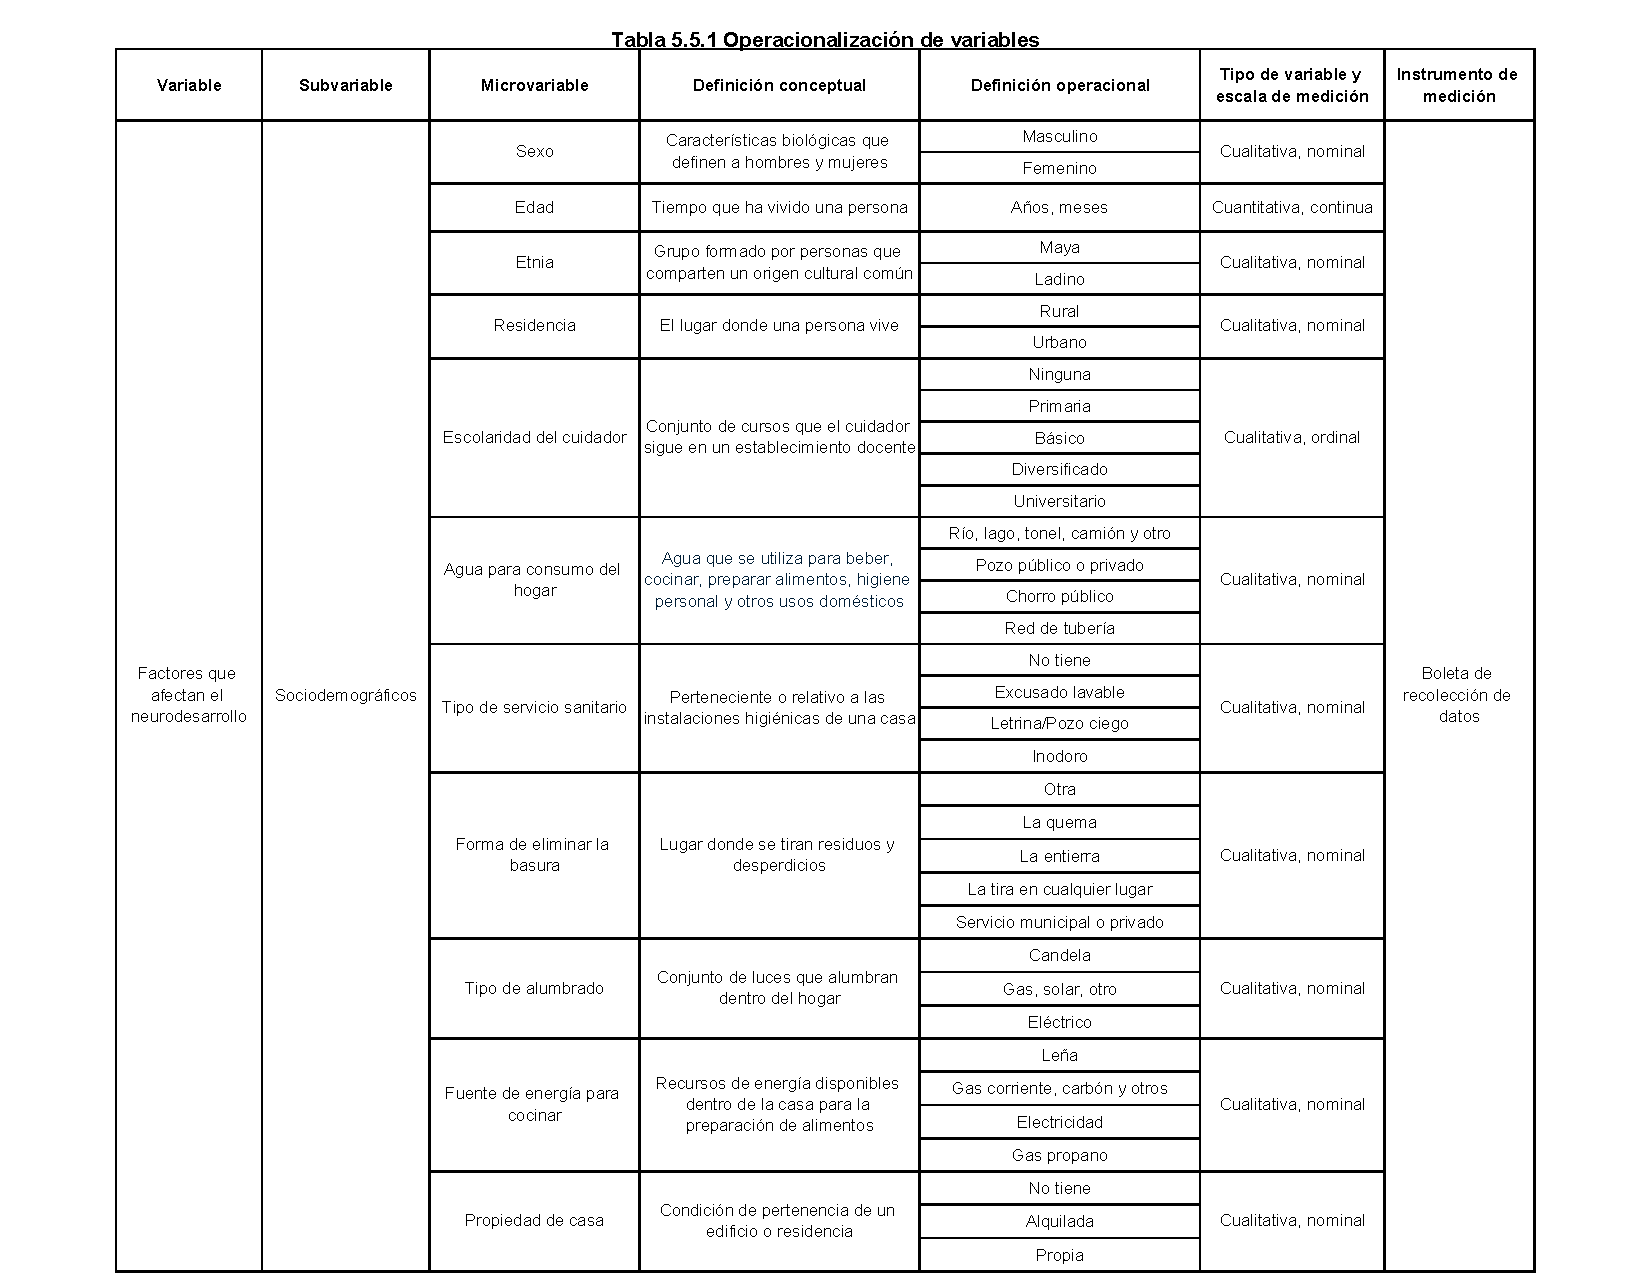
\includepdf[scale=0.90,landscape=true,pages=-,pagecommand={\thispagestyle{plain}}]{OpVariables.pdf}

\section{Hipótesis}
	\begin{enumerate}
		\item Hipótesis nula (H0): No existe una asociación significativa entre
		factores sociodemográficos, condiciones económicas, interacción
		familiar, exposición a dispositivos electrónicos, antecedentes médicos
		perinatales y postnatales, y el riesgo en el neurodesarrollo de niños
		menores de 5 años en servicios de atención primaria de Quetzaltenango.
		\item Hipótesis alternativa (H1): Existe una asociación significativa
		entre factores sociodemográficos, condiciones económicas, interacción
		familiar, exposición a dispositivos electrónicos, antecedentes médicos
		perinatales y postnatales, y el riesgo en el neurodesarrollo de niños
		menores de 5 años en servicios de atención primaria de Quetzaltenango.
	\end{enumerate}

\section{Técnicas de recolección de información e instrumentos de medición}
	\begin{enumerate}
		\item Técnicas de recolección de información: Para llevar a cabo este
		estudio de cohorte prospectivo, se implementarán las siguientes fases:
	\begin{enumerate}
		\item Fase preliminar (Febrero de 2025):
		Se obtuvieron los permisos correspondientes a las autoridades de salud
		del departamento de Quetzaltenango para acceder a los servicios de
		atención primaria seleccionados. Se determinaron estrategias para
		garantizar la uniformidad en la recolección de los datos entre los
		investigadores.
		\item Fase de recolección de datos:
		Se identificarán y reclutarán niños menores de 5 años que cumplan con
		los criterios de inclusión en los servicios de atención primaria
		participantes. Tras obtener el consentimiento informado de los padres o
		tutores, se realizará:
			\begin{itemize}
			\item Evaluación basal del neurodesarrollo mediante la aplicación
			del \asq, seleccionando la versión específica según la edad del
			niño.
			\item Aplicación de un cuestionario estructurado para recolectar
			información sobre factores potencialmente asociados al
			neurodesarrollo.
			\end{itemize}
		\item Fase de clasificación y análisis:
		Los resultados de cada niño serán evaluados conforme al
		puntaje obtenido en el \asq\
		y clasificados en tres categorías:
			\begin{itemize}
			\item Desarrollo típico: puntaje en el área blanca, indicativo de
			un desarrollo acorde a su edad.
			\item Requiere monitoreo: puntaje en el área gris, señalando
			habilidades ligeramente por debajo del promedio.
			\item Retraso en el desarrollo: puntaje en el área negra,
			sugiriendo la necesidad de intervención especializada.
			\end{itemize}
		Se analizarán las asociaciones entre los factores de exposición
		identificados y los resultados de neurodesarrollo en la evaluación.
	\end{enumerate}
	\item Instrumentos de recolección de información
	Para este estudio de cohorte prospectivo, se emplearán los siguientes
	instrumentos:
		\begin{itemize}
		\item \asq: Adaptado al idioma español y ajustado por edad. Esta
		herramienta validada de tamizaje del desarrollo identifica riesgos de
		problemas de neurodesarrollo en niños de 2 a 66 meses. Será aplicado
		por los investigadores con información proporcionada por los padres o
		tutores y mediante observación directa de actividades específicas.
		El \asq\ evalúa cinco áreas del desarrollo: comunicación, motricidad
		gruesa, motricidad fina, resolución de problemas, habilidades
		socioindividuales.

		\item Cuestionario de factores de exposición: Instrumento estructurado
		diseñado específicamente para este estudio que recopilará información
		sobre:
				\begin{itemize}
					\item Variables sociodemográficas (edad, sexo, etnia, nivel
					educativo de los padres)
					\item Variables económicas (empleo de los padres, acceso a
					seguridad social)
					\item Variables de interacción familiar (tiempo de juego,
					disponibilidad de juguetes)
					\item Variables médicas (prematuridad, peso al nacer, tipo
					de parto, lactancia, estado nutricional, etc.)
				\end{itemize}
		\end{itemize}
\end{enumerate}

\section{Plan de análisis de datos}
\begin{enumerate}
	\item Preparación de los datos: Los datos en formato físico serán
	digitados para su uso en el software estadístico Rstudio y python con los
	paquetes numpy y pandas. Se realizará una limpieza de los datos para
	identificar y corregir posibles errores de entrada. Los puntajes obtenidos
	en cada área del desarrollo del \asq\ se convertirán a valores
	estadísticos. 
	
	\item Análisis descriptivo de datos de la cohorte completa: Se calcularán
	frecuencias y porcentajes de los diferentes factores de riesgo presentes en
	la población a estudiar. Se calcularán medidas de tendencia central como
	media, mediana, y desviación estándar de los puntajes del neurodesarrollo.

	\item Análisis comparativo de los resultados del \asq\ de la cohorte
	completa utilizando las siguientes herramientas estadísticas:
		\begin{itemize}
		\item Chi-cuadrado: para determinar si hay asociación significativa
		entre las variables categóricas y riesgo del retraso en el
		neurodesarrollo, se utilizará para evaluar factores de riesgo
		individuales y comparar con desarrollo normal versus desarrollo en
		riesgo.
		\item Análisis de variancia (ANOVA): para comparar medias de puntajes
		del neurodesarrollo en más de dos grupos diferentes de una misma
		categoría y determinar su variación, por ejemplo para evaluar el riesgo
		del neurodesarrollo en valores Z y medidas de tendencia central con
		el grado de escolaridad de los padres de los niños: ninguna, primaria,
		básico, diversificado, universitario.
		\end{itemize}

	\item Análisis de asociación de los resultados del \asq\ del grupo
	estudiado utilizando:
		\begin{itemize}
		\item Odds ratio (OR): para comparar las probabilidades de que se
		presente riesgo en el neurodesarrollo entre dos grupos diferentes.
		Por ejemplo para comparar si los niños con padres que tienen un trabajo
		formal o informal tienen mayor probabilidad o no, de presentar riesgo
		en el neurodesarrollo.
		\end{itemize}
	\item Presentación de resultados: se elaborarán tablas y gráficos
	apropiados con intervalos utilizando el software Rstudio y paquetes de
	CRAN como ggplot2 para análisis y creación de datos informativos.
\end{enumerate}

\section{Principios éticos en la investigación}
Esta investigación se adherirá a los principios éticos clave, tales como:
\begin{itemize}
	\item Consentimiento informado: explicando claramente los objetivos del
	estudio a los padres o tutores y obteniendo su autorización.

	\item Confidencialidad: los datos se mantendrán anónimos y se utilizarán 
	exclusivamente para fines de investigación.

	\item Beneficencia y no maleficencia: buscando maximizar beneficios
	potenciales sin causar daños a los participantes.

	\item El \asq\ es una herramienta validada, respaldada por evidencia
	científica y recomendada por instituciones como UNICEF para su uso en
	evaluación del neurodesarrollo infantil en servicios de atención de
	salud. \cite{UNICEFrespaldo}
\end{itemize}

\printbibliography
\end{document}
